\documentclass[byrevtex,amssymb,aps,pra,floatfix,letterpaper]{revtex4}
\usepackage{graphicx}
\usepackage{hyperref}
\bibliographystyle{apsrev}
\date{\today}
\pagestyle{plain}
\newcommand{\degree}[0]{$^\circ$}

\begin{document}

\title{Introduction to undergraduate physical chemistry laboratory}

\date{\today}

\maketitle

\section{Overview}
\label{sec1}

A brief overview of some important steps for performing an experiment is provided below.

\begin{itemize}
\item Before starting a new experiment, you must always read the laboratory notes for that experiment before coming to class. The instructor will discuss the experiment with you and highlight the safety precautions. If you don't know the experimental procedure, the instructor will not let you proceed with the experiment.
\item Follow the instructions exactly. If you need to modify the procedure, always discuss this first with the instructor.
\item Notes must be taken during each experiment (see \ref{sec3}). You must provide photocopies of your notes to the instructor who will also initial your originals.
\item Notify the instructor of any broken equipment or if you run out of a reagent.
\item After finishing an experiment, put all the chemicals and equipment back where they belong. Clean your desk and the balance.
\item Prepare the written laboratory report according to Sec. \ref{sec4}.
\end{itemize}

\noindent
Read the following sections so that you will be able to safely complete the experiments. Note that this PDF file contains hyperlinks that can be activated by clicking on the underlined link -word.

\section{Laboratory safety}
\label{sec2}
\noindent
The laboratory instructor will review the following safety rules and regulations with you and will point out the location and operation of the fire extinguisher, safety shower, eye wash, and other laboratory safety equipment available.\\

\noindent
\underline{The safety rules:}
\begin{enumerate}
\item While in the laboratory, you must wear approved safety goggles. Hair and easily combustible clothing must be confined at all times. No exceptions! It is recommended to wear a laboratory coat.
\item Do not smoke, eat, or drink in the laboratory.
\item Before beginning to work in the laboratory you should be familiar with the procedure you will be following, as well as with any special precautions or changes that the instructor may note. Report any unexpected events to the instructor.
\item No unauthorized experiments may be performed. Violators will be subject to severe disciplinary action.
\item Before leaving the laboratory wash your hands carefully.
\item In case of an accident, the laboratory instructor must be quickly summoned. Furthermore:
\begin{enumerate}
\item If you receive a chemical burn, immediately flood the area with cold water while another student summons the instructor.
\item Treatment for injuries may be obtained from the Student Health Center.
\item The laboratory instructior will complete the appropriate departmental accident report.
\end{enumerate}
\item Practical precautions when conducting experiments:
\begin{enumerate}
\item When cutting glass tubing or inserting tubing into stoppers, protect your hands by using a towel. Glass tubing should be lubricated with glycerol or water to aid insertion of the tubing into stoppers. To remove tubing from stoppers, cut the stoppers rather than trying to pull it out.
\item When heating or carrying out reactions in a test tube, never point the mouth of the tube at your neighbor or yourself. Do not heat anything in a closed container.
\item Never taste or smell a chemical unless instructed to do so.
\item When smelling a chemical, fan vapors toward your face and inhale \textit{cautiously}.
\item Never pour water into concentrated acid; slowly add the acid to the water with constant stirring in a pyrex beaker or flask, not in a graduated cylinder.
\item Never pipet liquids by mouth; use a suction bulb.
\item If objectional vapors are given off during an experiment, the experiment must be performed in a hood.
\item Unless instructed otherwise, flammable solvents with boiling points less than 100 $^\textnormal{o}$C must be heated, distilled, or evaporated on a steam bath, not over or near an open flame. Flammable solvents should be contained in flasks rather than in open beakers. Make sure that electrical heaters used are in good condition such that they do not introduce sparks or over heating.
\item Student are responsible for cleaning up all spilled chemicals, on the reagent shelves, in the hoods, and around the balances. Consult the instructor if uncertain about the method of clean up.
\item No chemicals should be disposed of in the sink unless instructed to do so. There are chemical solvent waste bottles in the hood. If chemicals are disposed in the sink, they should be washed down with ample water for several minutes. Materials such as broken glass and towels should be placed in the receptacles beneath the sinks or in a waste jar. If in doubt, ask the instructor.
\item Never dispose of sodium, potassium or any alkali metal in the sinks as they react violently with water (and some even with air)! Consult the instructor for the method of disposal.
\end{enumerate}
\end{enumerate}

\section{Preparation of the laboratory notes}
\label{sec3}

Your laboratory notebook is the primary record of your observations during the experiment. The central requirements for a notebook are completeness and comprehensibility, not organization and polish. Make the notes in such a way that others can read them too. Even though things may look obvious at the moment, they may not be so obvious after few weeks! Include at least the following in your laboratory notes:

\begin{itemize}
\item Your name, the name of the experiment and the date.
\item Your ``prelab'' preparations -- calculations of concentrations, required glassware etc.
\item The equipment used and reagents including their purities.
\item Include details about weighing of compounds, volumes of liquids, and the related errors. In the latter case the errors may originate, for example, from the accuracy of the volumetric flasks or pipettes used.
\item Results from the measurement. Remember to label the numerical information you write down. In many cases, it is preferable to present results in tabular form.
\item ``Unexpected'' events -- like switching to another buffer solution, drift in instrumental readings, etc.
\end{itemize}

\noindent
You will be asked to provide a photocopy of your laboratory notes to the instructor. Once the instructor has received the photocopy, he/she will sign your laboratory notes. The original laboratory notes must be submitted with each written laboratory report. \textit{The original notes will not be accepted without the instructor signature!} If the experiment involves computer data files, be sure to store your data on floppy diskettes or a USB memory stick and make backups. Remember to document the file names in your notes so that you will be able to connect the file names to the actual measurements later on. Note that your laboratory notes will also contribute to the overall grade.\\

\noindent
\textit{Note: If you loose your laboratory notes, you will not be able to write the laboratory report and you will have to do the experiment again}. 

\section{Preparation of a written laboratory report}
\label{sec4}

A written laboratory report plays an equally important role as the experiment itself. The experimental results are usually meaningless unless they are not analyzed and interpreted properly. Furthermore such reports must provide the important details how the experiment was carried out. A general rule is that you should think that you are writing to another chemist (perhaps another chemistry student) who should after reading the report understand the experimental procedure and the meaning of the results. Do not include excessive amount of information or directly copy the laboratory instructions. The laboratory report format (see below) corresponds loosely to that of scientific research papers and part of the excercise is to learn how to write such documents.

Every student must prepare their own written laboratory report, which should include the following sections: Abstract, Introduction, Experiment, Data analysis, Results, Discussion and Rererences. The abstract must be preceded by a title, author and the date of the experiment. All equations, tables and figures must be numbered in sequence. In addition, tables and figures must include a caption that describes their content. All figures must have clearly specified axes (i.e.., axis label and unit; for example, Wavelength (nm)). A brief overview of the required sections is given below.\\

\noindent
\textit{Itroduction}. A brief introduction that summarizes the theoretical background, and the objective
and approach of the experiment. (length typically $<$ 1 page)\\

\noindent
\textit{Experiment}. Describe the experimental setup and add notes of any special procedures that were
carried out. For any instruments used, provide either the manufacturer and model or a schematic drawing of the setup. Indicate the possible error sources and accuracies for each instrument used. Chemicals and their purities must also be reported. Overall, the level of detail must be sufficient for others to repeat an equivalent experiment. Do not include irrelevant information, like what size flasks were used in preparing the solutions etc. (length typically $<$ 1 page)\\

\noindent
\textit{Data analysis}. Explain how the results were calculated using the experimental data. This would typically include data fitting and the related error estimates. Note also any computer programs and additional tools that were used. Do not include your prelab calculations here. (length typically $<$ 1 page)\\

\noindent
\textit{Results}. This section should contain the results from the experiments and how they were analyzed. Be sure to include the
raw data in tabular form (or as graphs, if they take excessive amount of space). Remember that all numerical data must be supplied with proper units (SI) and accuracy. For example, you can first show the raw data and then proceed in describing the analysis and referring to the figures and tables. (length typically $<$ 2 pages of text; may be longer when figures and tables are included)\\

\noindent
\textit{Discussion}. Discuss your results and compare your results to literature values (theoretical and/or experimental), if available. 
If your results deviate from the literature values, explain why this is so and is the difference significant. Remember to include reference numbers in the text for any literature values used.\\

\noindent
\textit{References}. A list of references must be given, if the report references works of others. The reference numbers must follow the order they appear in the text. The format for book
references is:\\

\noindent
1. R. J. Silbey, R. A. Alberty, and M. G. Bawendi, ``Physical Chemistry (4th ed.)'', John Wiley \&
Sons, Inc., New York (2005).\\

\noindent
and for articles:\\

\noindent
1. R. C. Neuman, Jr., and V. Jonas, ``\textit{Studies of chemical exchange by nuclear magnetic
resonance. IX. Rotation about the amide bond in N,N-dimethylformamide}'', J. Org. Chem. 39, 925 (1974).\\

\noindent
\textit{Feedback} (optional). Include suggestions and feedback regarding the experiment. This will not affect the grading but simply helps the instructor to develop the course.

\section{Reporting magnitudes and units}
\label{sec5}

\subsection{Approximate and exact values}

Approximate values are known only with some given accuracy. For example, many experimentally obtained values are approximate. Calculations using approximate values will also yield approximate results. Exact values are known with infinite precision. Examples of exact values are mathematical constants and many discrete variables such as the number of measurements, for example.

\subsection{Number of significant digits}

For exact values, all digits, that are required for communicating the numerical value exactly, are significant. For example, 175.5 has four significant digits and 1.2340 has five significant digits. In general, inclusion of the last zero indicates that the last digit is known to be zero. The number 3.141 $\times$ 10$^{-4}$ has four significant digits. Another way of writing this is 0.0003141. The zeros on the left of the number are not considered as significant digits.

For approximate values, the number of \href{http://en.wikipedia.org/wiki/Significant_figures}{\underline{significant digits}} tells us how accurately the value is known. For example, if we report an experimental result that has a value of 1.230, the accuracy of the measurement is communicated through the inclusion of the significant digits (four digits). How do we determine the last significant digit? One common practice is to define the last significant digit so that the maximum error in the digit can be 15 units at most. Lets consider an example. A measurement was carried out and a numerical value of 3.3245867 was obtained with an error of $\pm$ 0.000262. For the first four digits on the left, the uncertainty is zero units. For the fifth digit (5) the error is two units, which is still less than 15. However, for the sixth digit (8) the error is already 26 units (the leading digit in the error now counts), which is greater than 15. Thus this is the last digit that should be kept in the result. The error should also be rounded with the same accuracy as the value itself. The result should therefore be written as 3.32459 $\pm$ 0.0003. The number of significant digits is five. In another example 34.453 $\pm$ 0.148 should be reported as 34.45 $\pm$ 0.15 with four significant digits. Note the rounding from 0.148 to 0.15 when considering the units.

\subsection{Rounding of numbers}

In these experiments, it is sufficient to use the following \href{http://en.wikipedia.org/wiki/Rounding}{\underline{rounding conventions}}:

\begin{enumerate}
\item If the first digit to be discarded is less than 5, the last significant digit will appear as it is.
\item If the first digit to be discarded is 5 or larger, the last significant digit will be increased by one.
For example, 0.43 could be rounded to 0.4 and 0.45 to 0.5.
\end{enumerate}

\noindent
Note: The above is not strictly speaking correct. Why?

\subsection{The scientific notation}

In the \href{http://en.wikipedia.org/wiki/Scientific_notation}{\underline{scientific notation}} the base number and the exponent are written separately. For example, 3014.15 would be written in the scientific notation as 3.01415 $\times$ 10$^3$. Here 3.01415 is called the coefficient and it has to be a number greater than or equal to 1 and less than 10. The use of
scientific notation is preferred because the prefixes indicating powers of ten can be used to
simplify the exponent. For example, 10$^3$ would correspond to k (kilo) -- see Table \ref{table0} for a complete list.

\begin{table}[!htp]
\caption{Prefixes indicating the powers of ten.}
\begin{tabular}{l@{\extracolsep{0.5cm}}l@{\extracolsep{0.5cm}}l@{\extracolsep{1cm}}l}
 & & & \\
Prefix & Power & Prefix & Power\\
\cline{1-4}\\
exa (E) & 10$^{18}$ & atto (a) & 10$^{-18}$\\
peta (P) & 10$^{15}$ & femto (f) & 10$^{-15}$\\
tera (T) & 10$^{12}$ & pico (p) & 10$^{-12}$\\
giga (G) & 10$^9$ & nano (n) & 10$^{-9}$\\
mega (M) & 10$^6$ & micro ($\mu$) & 10$^{-6}$\\
kilo (k) & 10$^3$ & milli (m) & 10$^{-3}$\\
hecto (h) & 10$^2$ & centi (c) & 10$^{-2}$\\
deca (da) & 10$^1$ & deci (d) & 10$^{-1}$\\
\end{tabular}
\label{table0}
\end{table}

\subsection{Units}

A scientific quantity is not complete unless both the value and the unit are given. \href{http://en.wikipedia.org/wiki/SI}{\underline{SI units}} should be used in most cases. A list of SI units as well as the derived units are given tables \ref{table1}, \ref{table2} and \href{http://physics.nist.gov/cuu/Constants/}{http://physics.nist.gov/cuu/Constants/}.
\href{http://en.wikipedia.org/wiki/Conversion_of_units}{\underline{Conversion}} between SI and other unit systems are given Tables \ref{table3} and \ref{table4}. Some constants relevant to physical chemistry are listed in Table \ref{table4a} in SI units. For a more complete table, see Ref. \cite{OSTERMAN}.

\begin{table}[!htp]
\caption{SI units are an international standard (MKS; 1960).}
\begin{tabular}{l@{\extracolsep{0.5cm}}l@{\extracolsep{0.5cm}}l@{\extracolsep{1cm}}l}
 & & & \\
Quantity & Unit & Symbol & Definition\\
\cline{1-4}\\
length    &          meter &   m   &   Fixed to speed of light\\
mass      &          kilogram & kg  &   Weight of a reference cylinder\\
time      &          second  & s  &    Fixed to Cs radiative lifetime\\
current   &          ampere &  A  &    Fixed to current in reference system\\
temperature  &       kelvin &  K   &   0 K = absolute zero, 273.16 K = triple point of H$_2$O\\
luminous intensity &  candela &  cd  &   Fixed to a black-body reference\\
amount of substance & mole  &    mol &  The number of $^{12}$C atoms in 0.012 kg.\\
 & & & Avogadro's constant gives the number of molecules in one mole;\\
 & & & $N_A$ = 6.022137 $\times$ 10$^{23}$ mol$^{-1}$\\
\end{tabular}
\label{table1}
\end{table}

\begin{table}[!htp]
\caption{Derived units based on SI units.}
\begin{tabular}{l@{\extracolsep{0.5cm}}l@{\extracolsep{0.5cm}}l@{\extracolsep{1cm}}l}
 & & & \\
Quantity & Unit & Symbol & Definition\\
\cline{1-4}\\
force    &       newton  & N & 1 N = 1 kg m s$^{-2}$\\
energy   &       joule   & J &  1 J = 1 kg m$^2$ s$^{-2}$\\
electric charge & coulomb & C   &    1 C = 1 As\\
pressure  &      pascal  & Pa  & 1 Pa = 1 N m$^{-2}$\\
magnetic field & tesla  & T & 1 T = 1 kg s$^{-2}$ A$^{-1}$\\
frequency &      hertz  & Hz &  1 Hz = 1 s$^{-1}$\\
power     &      watt   & W &  1 W = 1 J s$^{-1}$\\
voltage   &      volt  &  V & 1 V = 1 W A$^{-1}$\\
resistance & ohm & $\Omega$  &    1 $\Omega$ = V A$^{-1}$\\
\end{tabular}
\label{table2}
\end{table}

\begin{table}[!htp]
\caption{Derived units based on SI units.}
\begin{tabular}{l@{\extracolsep{1cm}}l@{\extracolsep{2cm}}l}
 & & \\
Non-SI unit & SI unit & Conversion factor\\
\cline{1-3}\\
\AA ngstr\"om (\AA) & meter (m) & 1 \AA = 10$^{-10}$ m\\
inch (in)  &  meter (m)  &   1 in = 2.54 cm = 0.0254 m\\
foot (ft)  &  meter (m)  &   1 ft = 12 in = 0.3048 m\\
mile (mi)  &  meter (m)  &   1 mi = 5280 ft = 1609.344 m\\
AMU        &  kilogram (kg) & 1 AMU = 1.66054 $\times$ 10$^{-27}$kg\\
eV    &       joule (J) & 1 eV = 1.602177 $\times$ 10$^{-19}$ J\\
cal   &       joule (J) &  1 cal = 4.1868 J\\
torr (Hgmm) &       pascal (Pa) & 1 torr = 1.33322 $\times$ 10$^2$ Pa\\
atmospheres (atm) & pascal (Pa) & 1 atm = 1.01325 $\times$ 10$^5$ Pa\\
bar      &         pascal (Pa) & 1 bar = 10$^5$ Pa\\
psi      &        pascal (Pa) & 1 psi = 6.8948 $\times$ 10$^3$ Pa\\
gauss (G)  &       tesla (T) & 1 G = 10$^{-4}$ T\\
\end{tabular}
\label{table3}
\end{table}

\begin{table}[!htp]
\caption{Common conversion factors. For Kelvin units, the energy corresponds to $kT$. Note also that 1 K = 3.1669 $\times$ 10$^{-6}$ Hartree (atomic units; a.u.) or 1 eV = 27.2114 Hartree. To get J mol$^{-1}$ or kcal mol$^{-1}$, multiply by Avogadro's number $N_A$. For example, 1 eV = 1.602177$\times$10$^{-19}$ J and 1 atm = 760 torr.}
\begin{tabular}{l@{\extracolsep{0.5cm}}l@{\extracolsep{0.5cm}}l@{\extracolsep{0.5cm}}l@{\extracolsep{0.5cm}}l}
 & & & & \\
\underline{Mass -- Energy}\\
 & & & & \\
kg & u & J & eV & \\
\cline{1-4}\\
1 & 6.022137 $\times$ 10$^{26}$ & 8.987552 $\times$ 10$^{16}$ & 5.609586 $\times$ 10$^{35}$\\
1.660540 $\times$ 10$^{-27}$ & 1 & 1.492419 $\times$ 10$^{-10}$ & 9.314943 $\times$ 10$^8$\\
1.112650 $\times$ 10$^{-17}$ & 6.700531 $\times$ 10$^9$ & 1 & 6.241506 $\times$ 10$^{18}$\\
1.782663 $\times$ 10$^{-36}$ & 1.073544 $\times$ 10$^{-9}$ & 1.602177 $\times$ 10$^{-19}$ & 1\\
& & & & \\
\underline{Spectroscopic units}\\
& & & & \\
Hz & cm$^{-1}$ & Ry & eV\\
\cline{1-4}\\
1 & 3.335641 $\times$ 10$^{-11}$ & 3.039660 $\times$ 10$^{-16}$ & 4.135669 $\times$ 10$^{-15}$\\
2.99792458 $\times$ 10$^{10}$ & 1 & 9.112671 $\times$ 10$^{-6}$ & 1.239842 $\times$ 10$^{-4}$\\
3.289842 $\times$ 10$^{15}$ & 1.097373 $\times$ 10$^5$ & 1 & 1.360570 $\times$ 10$^1$\\
2.417988 $\times$ 10$^{14}$ & 8.065541 $\times$ 10$^3$ & 7.349862 $\times$ 10$^{-2}$ & 1\\
& & & & \\
\underline{Energy}\\
& & & & \\
K & kWh & kcal & J & eV\\
\cline{1-5}\\
1 & 3.83516 $\times$ 10$^{-30}$ & 3.298 $\times$ 10$^{-27}$ & 1.38066 $\times$ 10$^{-23}$ & 8.61739 $\times$ 10$^{-5}$\\
2.60745 $\times$ 10$^{29}$ & 1 & 8.598 $\times$ 10$^2$ & 3.60000 $\times$ 10$^6$ & 2.24694 $\times$ 10$^{25}$\\
3.0325 $\times$ 10$^{26}$ & 1.1630 $\times$ 10$^{-3}$ & 1 & 4.1868 $\times$ 10$^3$ & 2.6132 $\times$ 10$^{22}$\\
7.24292 $\times$ 10$^{22}$ & 2.77778 $\times$ 10$^{-7}$ & 2.388 $\times$ 10$^{-4}$ & 1 & 6.241506 $\times$ 10$^{18}$\\
1.16045 $\times$ 10$^4$ & 4.45049 $\times$ 10$^{-26}$ & 3.827 $\times$ 10$^{-23}$ & 1.602177 $\times$ 10$^{-19}$ & 1\\
& & & & \\
\underline{Pressure}\\
& & & & \\
Pa & bar & kp / cm$^2$ & torr (mmHg) & atm\\
\cline{1-5}\\
1 & 10$^{-5}$ & 1.020 $\times$ 10$^{-5}$ & 7.5006 $\times$ 10$^{-3}$ & 9.869 $\times$ 10$^{-6}$\\ 
10$^5$ & 1 & 1.020 & 7.5006 $\times$ 10$^2$ & 9.869 $\times$ 10$^{-1}$\\
9.807 $\times$ 10$^4$ & 9.807 $\times$ 10$^{-1}$ & 1 & 7.3556 $\times$ 10$^2$ & 9.678 $\times$ 10$^{-1}$\\
1.333 $\times$ 10$^2$ & 1.333 $\times$ 10$^{-3}$ & 1.360 $\times$ 10$^{-3}$ & 1 & 1.316 $\times$ 10$^{-3}$\\
1.013 $\times$ 10$^5$ & 1.013 & 1.033 & 760 & 1\\
\end{tabular}
\label{table4}
\end{table}

\begin{table}[!htp]
\caption{Some important constants relevant to physical chemistry.}
\begin{tabular}{l@{\extracolsep{0.5cm}}l@{\extracolsep{0.5cm}}l@{\extracolsep{1cm}}l}
 & & & \\
Name & Symbol & Value & Units\\
\cline{1-4}\\
Speed of light in vacuum & $c$ & 2.997925$\times$10$^8$ & m s$^{-1}$\\
Electron charge & $e$ & 1.602177$\times$10$^{-19}$ & C\\
Electron rest mass & $m_e$ & 9.109383$\times$10$^{-31}$ & kg\\
Proton rest mass & $m_p$ & 1.672622$\times$10$^{-27}$ & kg\\
Neutron rest mass & $m_n$ & 1.674927$\times$10$^{-27}$ & kg\\
Atomic mass unit & AMU & 1.660539$\times$10$^{-27}$ & kg\\
Gravitation constant & $g$ & 9.80665 & m s$^{-1}$\\
Vacuum permittivity & $\epsilon_0$ & 8.854188$\times$10$^{-12}$ & F m$^{-1}$\\
Planck's constant & $h$ & 6.626069$\times$10$^{-34}$ & J s$^{-1}$\\
Planck's constant / 2$\pi$ & $\hbar$ & 1.054572$\times$10$^{-34}$ & J s$^{-1}$\\
Boltzmann's constant & $k$ or $k_B$ & 1.380651$\times$10$^{-23}$ & J K$^{-1}$\\
Gas constant ($N_a\times k$) & $R$ & 8.31447 & J mol$^{-1}$ K$^{-1}$\\
 & & 0.0831447 & L bar mol$^{-1}$ K$^{-1}$\\
 & & 0.0820574 & L atm mol$^{-1}$ K$^{-1}$\\
 & & 62.3637 & L torr $^{-1}$ K$^{-1}$\\
Avogadro number & $N_A$ & 6.022142$\times$10$^{23}$ & mol$^{-1}$\\
Faraday constant ($N_A\times e$) & $F$ & 9.648534$\times$10$^4$ & C mole$^{-1}$\\
Magnetogyric ratio for protons & $\gamma_H$ & 2.67522$\times$10$^8$ & s$^{-1}$ T$^{-1}$\\
\end{tabular}
\label{table4a}
\end{table}

\section{Error analysis}
\label{sec6}

Error analysis attempts to give reliable error bounds for a given approximate value. As most experimentally obtained results contain inevitable sources of error, it is necessary to be able to determine the errors involved in a consistent manner. For example, a balance or a pipet have their specified accuracy and therefore the use such an instrument in an experiment leads to an error in the quantities determined. Thus it is important to be aware of the error sources, their magnitudes and their effect on the overall experiment. A comprehensive discussion on error analysis relevant to physical chemistry can be found from Refs. \cite{MCBANE,TAYLOR}.

\subsection{Determination of accuracy}

As discussed earlier, an error bound specifies the interval where the accurate value resides with respect to its most probable value. For example, when measuring the thickness of a book with a regular ruler, we might observe it to be 1.55 cm thick within 0.05 cm. The 0.05 cm uncertainty originates from the accuracy of our ruler. Thus the real thickness of the book is somewhere between 1.50 cm and 1.60 cm. This usually expressed as 1.55 $\pm$ 0.05 cm. In general, for a variable $x$, the result should be given as:

\begin{center}
$<$the best value for $x>$ $\pm$ $<$the estimated error in $x$; denoted by $\delta x>$
\end{center}

\noindent
In the previous ``book example'', we can choose the error bound loosely enough that we can be
sure that the accurate value of the book thickness is in the specified interval. However, obviously
it should not be made excessively large because then it would loose its significance. In many
cases it is not obvious what value $\delta x$ should have and sometimes the error must be just simply
understood as a purely statistical quantity. In that context the ``best value'' is usually denoted as a
mean value. The measurements are thus sampling a distribution of values.

The \textit{relative error} can be defined as:

\begin{equation}
\label{eq1}
\textnormal{Relative error} = \frac{\delta x}{\overline{x}}
\end{equation}

\noindent
where the over bar indicates a mean value. The relative error accounts for the magnitude of the
quantity in the error. The relative error is usually reported in percent (\%) and for the previous
``book example'', we would have: 1.55 cm $\pm$ 3 \%. The relative error is dimensionless, unless it is
given in percent.

\subsection{Probability distributions}

There are several common probability distributions that are used in describing the spread of errors in measurements, for example, the \href{http://en.wikipedia.org/wiki/Normal_distribution}{\underline{normal distribution}}, the \href{http://en.wikipedia.org/wiki/Student's_t-distribution}{\underline{Student's t-distribution}} and the \href{http://en.wikipedia.org/wiki/Poisson_distribution}{\underline{Poisson distribution}}. Depending on the error sources involved, the measured values follow the appropriate distribution around some mean value. This error distribution can be constructed, for example, by carrying out repeated measurements of the observable and plotting the results on a graph.

In most scientific experiments, the measured values follow the \href{http://en.wikipedia.org/wiki/Normal_distribution}{\underline{the normal distribution}} (also called Gaussian distribution). This is essentially predicted by the \href{http://en.wikipedia.org/wiki/Central_limit_theorem}{\underline{central limit theorem}}, which states that small random fluctuations in a large number of variables add up to a common normal distribution regardless of the original distributions of the variables. The normal distribution is defined as in Eq. (\ref{eq1a}):

\begin{equation}
\label{eq1a}
P(x; \mu, \sigma) = \frac{1}{\sqrt{2\pi}\sigma}e^{-\frac{1}{2}\left(\frac{x-\mu}{\sigma}\right)^2}
\end{equation}

\noindent
where $\mu$ is the \textit{mean} and $\sigma$ is the \href{http://en.wikipedia.org/wiki/Standard_deviation}{\underline{standard deviation}} of the distribution (i.e., the width). An example of normal distribution is shown in Fig. \ref{figgauss}. In this distribution, about 68\% of the results are within $\mu - \sigma$ and $\mu + \sigma$.

\begin{figure}[!htp]
\vspace{0.5cm}
\begin{center}
\includegraphics[scale=0.4]{figgauss}
\caption{Normal distribution with $\mu = 5$ and $\sigma = 1$.}
\label{figgauss}
\end{center}
\end{figure}

The \href{http://en.wikipedia.org/wiki/Student's_t-distribution}{\underline{Student's t-distribution}} is a probability distribution that arises in the problem of estimating the mean of a normally distributed population when the sample size is limited or the standard deviation of the population is unknown. It is also the basis of the popular Student's t-tests for the statistical significance of the difference between two sample means, and for confidence intervals for the difference between two population means. Student's t-distribution approaches the normal distribution when the number of samples is large.

The \href{http://en.wikipedia.org/wiki/Poisson_distribution}{\underline{Poisson distribution}} is a distribution function that usually arises from counting events. Eventhough the distribution itself is continuous, the corresponding experimental data is discrete. Eq. (\ref{eq1b}) gives the expression for this distribution:

\begin{equation}
\label{eq1b}
P(x; \mu) = \frac{\mu^x}{x!}e^{-\mu}
\end{equation}

\noindent
where $\mu$ is the average of the distribution. Note that there is no parameter defining the width. When $\mu<<1$ the distribution looks like a decaying exponential function and when $\mu>>1$ it remebles the normal distribution.

\subsection{Application of error analysis}

If two ``identical'' measurements for a given quantity do not yield the same result, there is
difference between the obtained values. Numerically the difference between the results is
obtained by subtracting the values from each other. For example, if two students measure the
voltage of a given battery as 15 $\pm$ 2 V and 24 $\pm$ 3 V, the difference between the results is 24 V $-$
15 V = 9 V (always a non-negative number). If we consider the error bounds given, we can
immediately see that the difference is significant because the two results are not within the
bounds. Therefore we can say that one of the measurements must be incorrect. If the results had
been 16 $\pm$ 8 V and 25 $\pm$ 9 V, the difference would be insignificant because the two results are
within the given bounds. Thus both measurements in this case are correct.

In physical chemistry laboratory work some quantities of interest are measured and
compared to the results obtained by others. In order to carry out the comparison, it is necessary to
consider both the value and the associated error bound. Let's consider an adiabatic bomb
calorimeter experiment as an example. The experiment gave the heat of combustion for salicyclic
acid as $-$24.4 $\pm$ 0.4 kJ/g. The corresponding literature value is 24.77 $\pm$ 0.02 kJ/g. When comparing
the two values, the error bounds must also be considered. In this case the experiment can be
considered successful because the result is within the proper bounds.

\subsection{Types of errors}

Errors can be classified as \textit{systematic errors}, \textit{random errors} or \textit{coarse errors}. \href{http://en.wikipedia.org/wiki/Systematic_error}{\underline{Systematic errors}} are characterized by their tendency to be in one direction only, either positive or negative. For example, if a ruler is worn at one end, it will introduce a constant error. Improper instrument calibration causes systematic errors. Systematic errors are usually more important than random errors and they are generally much more difficult to deal with. Although systematic errors cannot be eliminated entirely, they can be minimized by careful experimental design and by assuring that measurements can be traced to known standards.

Random errors, on the other hand, are produced by unaccounted for variations in experimental conditions or from small errors in making observations, such as estimating units of the smallest scale division. They tend to be scattered over a finite range of values. If assumptions are made about the distribution of random errors it is possible to use statistical methods to deal with them. The terms accuracy and precision are often used to distinguish between systematic and random errors. If a measurement has small systematic errors, it has high accuracy; if the measurement random errors are small, it has high precision.

In addition to systematic and random errors, there may be coarse errors related to the person carrying out the experiment. These include incorrect reading of meters, incorrect laboratory notes, careless work, sudden change in experimental conditions etc. Results from measurements subject to these errors must be discarded. If you have to discard a particular result, you must indicate this in your laboratory notebook.

\subsection{Mean value and standard deviation}

If repeated experiments carried out and yield the measured values $x_1, ..., x_n$, the average of the measurements should be reported:

\begin{equation}
\label{eq11}
\overline{x} = \frac{1}{n}\sum\limits_{i=1}^{n} x_i
\end{equation}

\noindent
where the overline denotes an average. The sample \href{http://en.wikipedia.org/wiki/Standard_deviation}{\underline{standard deviation}} of the set is given by:

\begin{equation}
\label{eq12}
s_x = \sqrt{\frac{1}{n-1}\sum\limits_{i=1}^{n}\left(x_i - \overline{x}\right)^2}
\end{equation}

\noindent
which characterizes the variability of the measurements. This estimate does not account for the
fact that our knowledge of the true value must increase as the number of measurements increases.
This is corrected in the standard deviation of the mean estimate:

\begin{equation}
\label{eq13}
\overline{s}_x = \frac{1}{\sqrt{n}}s_x
\end{equation}

\noindent
For example, if time is being measured and the following results are obtained: 15.1 s, 15.3 s, 15.1
s, and 15.2 s, we have for Eqs. (\ref{eq12}) and (\ref{eq13}):

\begin{eqnarray}
\label{eq14}
& s_x = \sqrt{\frac{\left(-0.075\textnormal{ s}\right)^2 + \left(0.125\textnormal{ s}\right)^2 + \left(-0.075\textnormal{ s}\right)^2 + \left(0.025\textnormal{ s}\right)^2}{3}} = 0.096\textnormal{ s}\\
\nonumber
& \overline{s}_x = \frac{0.096\textnormal{ s}}{\sqrt{4}} = 0.048\textnormal{ s}
\end{eqnarray}

\noindent
Thus the result of the measurement is (15.18 $\pm$ 0.05) s. If you are using the scientific notation, both the value and the uncertainty must have the same exponential part. Both parts must always be reported to the same number of decimal places.

A \href{http://en.wikipedia.org/wiki/Confidence_interval}{\underline{confidence interval}} is an interval estimate for a parameter obtained from experiments. Instead of estimating the parameter by a single value, an interval of likely estimates with some percentage is given. The higher the uncertainty in the parameter, the wider the interval will be. For example, in the normal distribution, the standard deviation of the mean corresponds to the 68\% confidence interval. In practice, it means that 68\% of the measurements fall in this interval, $\mu + \sigma$ and $\mu - \sigma$. Note that confidence interval is just another way of expressing how much error is involved in the experimental determination of some parameter.

\subsection{The law or error propagation}

Let $x, ..., z$ be measured quantities and the error bounds $\delta x, ..., \delta z$, which are independent and
random. The error in function $q = q(x, ..., z)$ can be obtained using the following formula
\cite{TAYLOR}:

\begin{equation}
\label{eq2}
\delta q = \sqrt{\left(\frac{\partial q}{\partial x}\times\delta x\right)^2 + ... + \left(\frac{\partial q}{\partial z}\times\delta z\right)^2}
\end{equation}

\noindent
This is called the \href{http://en.wikipedia.org/wiki/Error_propagation}{law of error propagation}. A qualitative way to understand Eq. (\ref{eq2}) is to
interpret the partial derivatives as differences (i.e., each term in the sum gives ($\Delta q)^2$) and then the
total error is then obtained by adding all the errors together. Consider the following example.\\

\noindent
\textit{Example.} Density of a liquid is given by $\rho = m / V$, where $\rho$ is the density, $m$ is the total mass of
the liquid and $V$ is the total volume. The following values were determined experimentally: $m =
21.34 \pm 0.01$ g and $V = 20.00 \pm 0.12$ cm$^3$. For the mass $m$ the error ($\delta m$) originates from the
accuracy of the balance used and for $V$ ($\delta V$) from the volumetric accuracy of the flask or pipet.
The error in density ($\delta\rho$) can now be obtained by using Eq. (\ref{eq2}):

\begin{equation}
\label{eq3}
\delta\rho = \sqrt{\left(\frac{\partial\rho}{\partial m}\times\delta m\right)^2 + \left(\frac{\partial\rho}{\partial V}\times\delta V\right)^2}
\end{equation}

\noindent
The required partial derivatives can be calculated as:

\begin{equation}
\label{eq4}
\frac{\partial\rho}{\partial m} = \frac{1}{V}\textnormal{ and }\frac{\partial\rho}{\partial V} = -\frac{m}{V^2} 
\end{equation}

\noindent
When these are inserted in Eq. (\ref{eq3}), we have:

\begin{equation}
\label{eq5}
\delta\rho = \sqrt{\left(\frac{\delta m}{V}\right)^2 + \left(-\frac{m\delta V}{V^2}\right)^2}
\end{equation}

\noindent
Now inserting $\delta m$ = 0.01 g and $\delta V$ = 0.12 cm$^3$, we get:

\begin{equation}
\label{eq6}
\delta\rho = \sqrt{\left(\frac{0.01\textnormal{ g}}{20.00\textnormal{ cm}^3}\right)^2 + \left(-\frac{21.34\textnormal{ g}\times0.12\textnormal{cm}^3}{\left(20.00\textnormal{ cm}^3\right)^2}\right)^2} = 0.000642\textnormal{~}\frac{\textnormal{g}}{\textnormal{cm}^3}
\end{equation}

\noindent
Thus the final result is then: $\rho$ = 1.067 $\pm$ 0.007 g cm$^{-3}$. Note that the main error arises from the
inaccuracy in determining the volume. If you can estimate the magnitudes of errors caused by
different variables, it is sometimes possible to simplify the error treatment by only considering the
major sources or error.

\subsection{Other error estimates}

In the previous error estimate, we assumed that all the errors $\delta x, ..., \delta z$ are random and
independent of each other. If this does not hold, we can still provide the following error estimate \cite{TAYLOR}:

\begin{equation}
\label{eq7}
\delta q \le \left|\frac{\partial q}{\partial x}\right|\delta x + ... + \left|\frac{\partial q}{\partial z}\right|\delta z
\end{equation}

\noindent
where $\left| \cdot \right|$ denotes an absolute value.

A simple error estimate can also be obtained by calculating the mean value of the maximum and minimum values for the function:

\begin{equation}
\label{eq8}
\delta q = \frac{q_{max} - q_{min}}{2}
\end{equation}

\noindent
For example, in the previous example this would give:

\begin{eqnarray}
\label{eq9}
\rho_{max} = \frac{m + \delta m}{v - \delta V} = \frac{\left(21.34 + 0.010\right)\textnormal{ g}}{\left(20.00 - 0.12\right)\textnormal{ cm}^3} = 1.0739\textnormal{ g cm}^{-3}\\
\nonumber
\rho_{min} = \frac{m - \delta m}{v + \delta V} = \frac{\left(21.34 - 0.010\right)\textnormal{ g}}{\left(20.00 + 0.12\right)\textnormal{ cm}^3} = 1.0601\textnormal{ g cm}^{-3}
\end{eqnarray}

\noindent
Now Eq. (\ref{eq8}) yields the following estimate:

\begin{equation}
\label{eq10}
\delta\rho = \frac{\left(1.0739 - 1.0601\right)\textnormal{ g cm}^{-3}}{2} = 0.007\textnormal{ g cm}^{-3}
\end{equation}

\noindent
In this case the estimate is exactly the same as was obtained by using Eq. (\ref{eq2}). This, however,
becomes a very laborious, if many variables and more complicated expressions are involved.

\subsection{Outliers}

If you observe that, for example, one of the data points appears to be completely out of line as compared to the other points, is it possible that there was some sort of mistake in this particular measurement? Maybe, but before discarding or keeping the point, you should consider the following: 1) check your calculations for this point, 2) repeat the measurement for that point if possible, or 3) classify the point as \href{http://en.wikipedia.org/wiki/Outlier}{\underline{outlier}} using statistical methods. In the latter case, given that the experiment is governed by the normal distribution and there is just one outlier point, it is possible to use the $Q$ test \cite{MCBANE}:

\begin{equation}
\label{eq10a}
Q = \frac{x_{suspect} - x_{closest}}{x_{suspect} - x_{farthest}}
\end{equation}

\noindent
where $x_{suspect}$ is the outlier point value, $x_{closest}$ is the closest $x$ value to the outlier and $x_{farthest}$ is the point farthest away from the outlier. For 90\% confidence level, if the value of $Q$ exceeds: 0.941 ($N$ = 3), 0.765 ($N$ = 4), 0.642 ($N$ = 5), 0.560 ($N$ = 6), 0.507 ($N$ = 7), 0.468 ($N$ = 8), 0.437 ($N$ = 9) and 0.412 ($N$ = 10), you may discard the point \cite{MCBANE}. Here $N$ denotes the number of measured points. Note that if you discard an outlier point, you will need to recalculate averages, standard deviations, etc. without the outlier point.

\section{Graphs}

When preparing a graph, the following issues should be kept in mind:

\begin{itemize}
\item Graphs must always have a name.
\item A graph must be drawn with coordinate axes where the horizontal axis represents the independent variable (``$x$'') and the horizontal axis the dependent variable (``$f(x)$'').
\item The coordinate axes must be given meaningful names and proper units must be indicated on them (in the middle or at the end of the axes).
\item The axis labels must be chosen in such a way that the values of the data points are easy to read.
\item The data points must be clearly marked in the graph. It is suggested that either black dots or crosses are used.
\item If error bars are available for the individual points, they should be indicated in the graph by drawing a vertical segment on the data points (see Fig. \ref{fig1}).
\item When drawing a curve that connects the data points, this should be done smoothly ignoring the random errors in points. Preferably a least squares fit should be provided.
\item If the errors in slopes are to be demonstrated graphically, a pair dotted of error lines should be drawn. They correspond to maximum and minimum values for the slope. Note that this method can be used for obtaining the errors graphically as well.
\item If the errors in points of intercept are to be demonstrated graphically, a set of additional lines should be drawn. The intercepts of the error lines correspond to the minimum and maximum values. Note that this method can be used for obtaining the errors graphically as well. The most common way is to obtain the errors from the least squares fit method (next section).
\item The statistical prediction bands (95\%, for example) can be included in the graph as shown in Fig. \ref{fig2}.
\end{itemize}

\begin{figure}[!htp]
\begin{center}
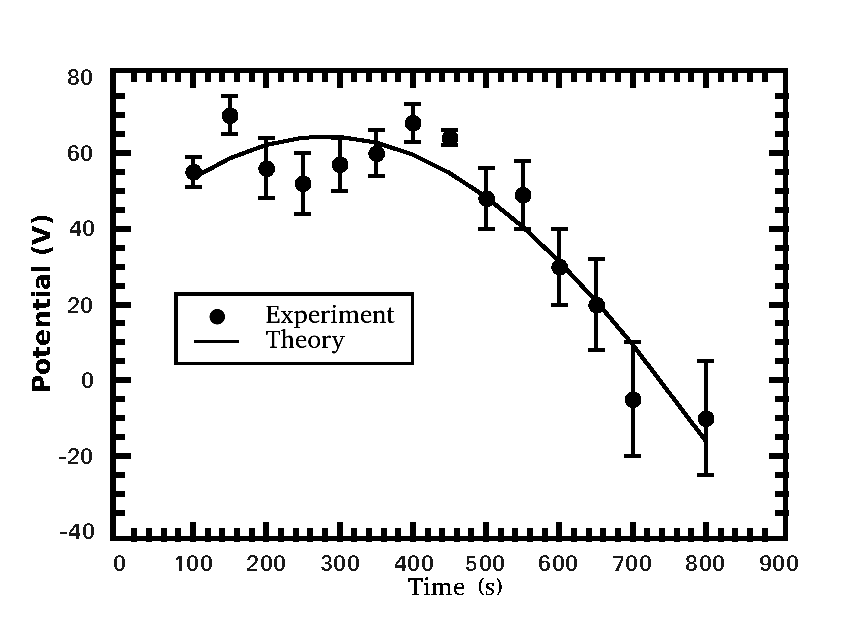
\includegraphics[scale=0.5]{graph1}
\caption{A graph demonstrating the use of error bars for data points (black dots). The continuous
line represents the results from a least squares fitting procedure.}
\label{fig1}
\end{center}
\end{figure}

\begin{figure}[!htp]
\begin{center}
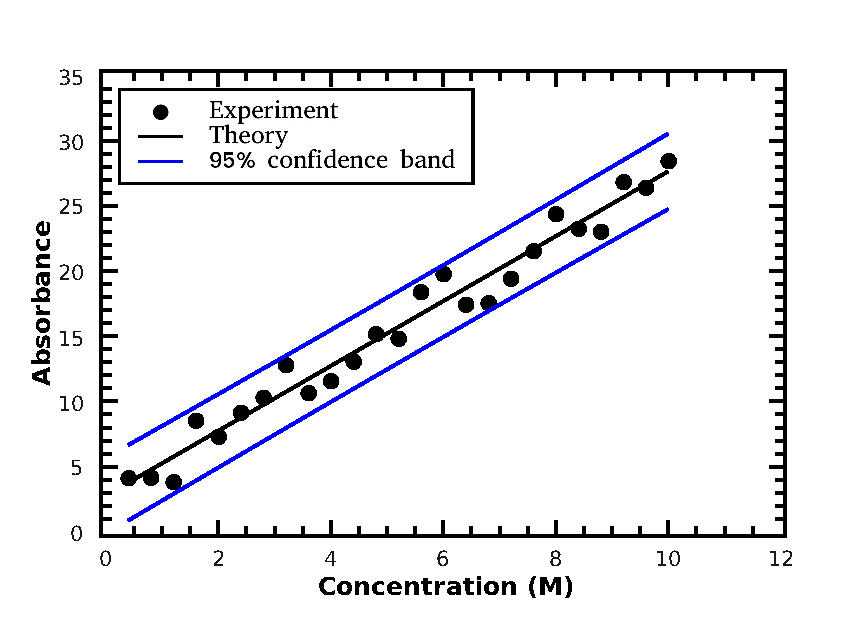
\includegraphics[scale=0.5]{graph2}
\caption{Experimental data points (circles) showing linear behavior. The solid line was obtained by the linear least square fitting procedure. The data points deviate slightly from strictly linear behavior because of the experimental uncertainty. The confidence band lines show the 95\% interval.}
\label{fig2}
\end{center}
\end{figure}

\section{The least squares method}
\label{sec7}

\subsection{The linear least squares method}
\label{sec7.1}

In physical chemistry mathematical models are usually developed to describe dependencies between different variables. For example, recall the \href{http://en.wikipedia.org/wiki/Beer-Lambert_law}{\underline{Beer-Lambert law}} used in UV/VIS spectroscopy:

\begin{equation}
\label{eq15}
A = \epsilon cl
\end{equation}

\noindent
where $A$ is the absorbance of a given species, $\epsilon$ is the molar absorption coefficient and $l$ is the length of the sample (\href{http://en.wikipedia.org/wiki/Optical_path_length}{\underline{optical path length}}). If we had a set of points consisting of sample concentrations and \href{http://en.wikipedia.org/wiki/Absorbance}{\underline{absorbances}}, we should be able to obtain a value and the error bounds for $\epsilon$ (the sample length is assumed to be known). If the data points are plotted, the points should fall on a straight line (within the accuracy of the measurement) as shown in Fig. \ref{fig2}. In the following we will outline the \href{http://en.wikipedia.org/wiki/Linear_regression}{\underline{linear least squares method}} (also called ``linear regression'') and show how it can be applied in fitting a given mathematical model to a set of experimental data.

First we consider the linear case (i.e., the function is of the form $y = kx + b$). If the data
points are denoted by $(x_1, y_1), ..., (x_n, y_n)$, the least squares error function is:

\begin{equation}
\label{eq16}
\chi^2(k,b) = \sum\limits_{i=1}^{n}\left(y(x_i; k, b) - y_i\right)^2 = \sum\limits_{i=1}^{n}\left(kx_i + b - y_i\right)^2
\end{equation}

\noindent
The function in Eq. (\ref{eq16}) tells how much overall deviation there is between the data and the function. The error function depends on two parameters $k$ and $b$. In order to find the best values for the parameters, it is necessary to minimize the error function $\chi^2(k,b)$ with respect to $k$ and $b$. Note that sometimes weighting constants $w_i$ may be added to Eq. (\ref{eq16}) to vary to the significance of the points, above we have chosen $w_i \equiv 1$.

The exact derivation of the solution is not given here (see, for example, Ref. \cite{NUMREP}) but the results can be summarized as:

\begin{eqnarray}
\label{eq17}
& & k = \frac{S_{xx}S_y - S_xS_{xy}}{\Delta}\textnormal{ and }b = \frac{nS_{xy}-S_xS_y}{\Delta}\\
\nonumber
& & \textnormal{where }S_x = \sum\limits_{i=1}^{n} x_i\textnormal{, }S_y = \sum\limits_{i=1}^{n} y_i\textnormal{, }S_{xx} = \sum\limits_{i=1}^{n} x_i^2\textnormal{, } S_{xy} = \sum\limits_{i=1}^{n} x_iy_i\textnormal{ and }\Delta = nS_{xx} - S_x^2
\end{eqnarray}

\noindent
When the \href{http://en.wikipedia.org/wiki/Error_propagation}{\underline{law of error propagation}} is applied, we obtain the following \href{http://en.wikipedia.org/wiki/Standard_error_\%28statistics\%29}{standard error} estimates for $k$ and $b$:

\begin{equation}
\label{eq18}
\delta k = \sqrt{\frac{S_{xx}}{\Delta}}\textnormal{ and }\delta b = \sqrt{\frac{n}{\Delta}}
\end{equation}

\noindent
The overall quality of the fit can be estimated from the \href{http://en.wikipedia.org/wiki/Coefficient_of_determination}{\underline{correlation coefficient}}:

\begin{equation}
\label{eq19}
r^2 = 1 - \frac{\chi^2}{\sum\limits_{i=1}^{n}\left(y_i - \overline{y}\right)^2}
\end{equation}

\noindent
where the overline denotes an average. If the correlation coefficient is close to one, the fit is
excellent. However, if the $r^2$ is close to zero, the data doesn’t fit the function, which means that the
procedure failed. All the calculations can, in principle, be carried out by hand, but for large
number of samples this becomes a tedious task. There are computer programs available for least
squares fitting.

\subsection{Application of the linear least squares method on some ``non-linear'' functions}

The linear least squares method can be applied to some non-linear functions as well provided that
one can find a suitable transformation. For example, consider the following non-linear function:

\begin{equation}
\label{eq20}
y = Ae^{Bx}
\end{equation}

\noindent
where $A$ and $B$ are parameters to be fitted. The linear least squares method cannot be applied
directly because the function in Eq. (\ref{eq20}) is non-linear. However, if natural logarithms are taken on
both sides of the equation, we get:

\begin{equation}
\label{eq21}
\underbrace{\ln(y)}_\textit{``y''} = \ln(Ae^{Bx}) = \ln(A) + \ln(e^{Bx}) = \underbrace{\ln(A)}_\textit{``b''} + \underbrace{Bx}_\textit{``kx''}
\end{equation}

\noindent
As indicated by the comments above, the equation becomes linear after this transformation. A
plot of $\ln(y)$ against $x$ will yield a straight line with a slope that equals $B$. In order to obtain $A$, a
natural logarithm of the point of interception must be taken. The linear least squares method can also be extended
to fit polynomial functions \cite{NUMREP}.

\subsection{The non-linear least squares method}

In non-linear least squares, the model function $y(x; p_i)$ in $\chi^2$ (see Eq. (\ref{eq16})) is non-linear. Here $p_i$'s are the model parameters to be optimized. In practice, this means that methods based on linear least squares method cannot be applied and the non-linear problem has to be solved by using general minimization methods. Examples of such optimization methods are the conjugate gradient, Newton and Levenberg-Marquardt methods \cite{NUMREP}. They require user to provide initial guesses for the model variables $p_i$ as well as various parameters that control the optimizion algorithm. Note that these methods may converge to local minimima, which may result in non-optimal fits. The general idea of these methods is that they calculate the gradient vector of $\chi^2$ at a given point and attempt to follow $-\nabla\chi^2$ to locate the minimum (for example, gradient, conjugate gradient, Newton, Levenberg-Marquardt \cite{NUMREP}). Typically this process will take several iterations to converge. The non-linear least squares can be easily extended to fit multiple data sets and models simultaneously using a set of shared parameters $p_i$. This situation is often encountered when fitting experimental concentration data to kinetic models. Error analysis in non-linear least squares is very tricky and accuarate error analysis would often require Monte Carlo simulations. However, in practice, it is assumed that the $\chi^2$ can be approximated by a linear function of the parameters near the minimum and that the measurement errors obey a normal distribution. In this case, the Hessian matrix (i.e., the 2nd derivative matrix) of $\chi^2$ can be used to obtain the obtain the standard errors for the parameters $\alpha_{ii}$ \cite{NUMREP}:

\begin{equation}
\label{eq22}
\alpha_{ii} = \sigma^2\left(
\begin{array}{ccc}
\frac{\partial^2 \chi^2}{\partial p_1^2} & ... & \frac{\partial^2 \chi^2}{\partial p_1p_n}\\
... & ... & ...\\
\frac{\partial^2 \chi^2}{\partial p_np_1} & ... & \frac{\partial^2 \chi^2}{\partial p_n^2}\\
\end{array}
\right)^{-1}
\end{equation}

\noindent
where the variance in measurements $\sigma^2$ is usually approximated as:

\begin{equation}
\label{eq22a}
\sigma^2 \approx \frac{\chi^2_{opt}}{m-n}
\end{equation}

\noindent
and $\chi^2_{opt}$ refers to $\chi^2$ evaluated at the optimimum values of $p_i$, $m$ is the total number of data points and $n$ is the number of parameters $p_i$. Note that the failure of the linearity assumption may lead to an unrealistically larger estimate of the errors. The standard errors $\alpha_{ii}$ can be used for providing confidence bands. For example, 95\% confidence band is given by:

\begin{equation}
\label{eq22b}
p_i - 1.95\alpha_{ii} \le p_i \le p_i + 1.95\alpha_{ii}
\end{equation}

\noindent
The above procedure has been implemented in the ``nlsq.mac'' and qtiplot programs.

\section{Common experimental techniques}
\label{sec8}

\subsection{Vacuum basics}

The three common vacuum ranges are low (above 10$^{-3}$ Torr), high (10$^{-3}$ - 10$^{-9}$ Torr) and ultra-high (below 10$^{-9}$ Torr; see \url{http://en.wikipedia.org/wiki/Ultra-high_vacuum}) vacuum. Each pressure range places its special requirements for the vacuum pumps, vacuum line, and the measurement of pressure. Note that it is not practically possible to create perfect vacuum and hence the use of word vacuum does not necessarily imply that it would be a perfect one.

\subsubsection{Vacuum pumps}

A \href{http://en.wikipedia.org/wiki/Vacuum_pump}{\underline{vacuum pump}} is a pump that removes gas molecules from a sealed volume in order to leave behind a partial \href{http://en.wikipedia.org/wiki/Vacuum}{\underline{vacuum}}. Vacuum pumps can be broadly catergorized into three classes:

\begin{itemize}
\item \textit{Positive displacement pumps}, which are based on the following pump cycle: expand to let gas flow through the inlet into the pump chamber, seal the chamber and finally exhaust by opening the chamber to the outlet of the pump (i.e., the exhaust). Examples of this type of pumps are: \href{http://en.wikipedia.org/wiki/Rotary_vane_pump}{\underline{rotary vane pump}} (``oil pump'', ``mechanical pump''; most common type; oil contamination problem; 2 stage pumps for improved vacuum), \href{http://en.wikipedia.org/wiki/Diaphragm_pump}{\underline{diaphragm pump}} (no oil contamination) and \href{http://en.wikipedia.org/wiki/Roots_blower}{\underline{roots pump}} (``booster pump''; extremely high pumping speeds). For example, two stage rotary vane pumps can produce vacuum down to 10$^{-3}$ Torr. Before operating a rotary vane pump, make sure that there is enough pump oil in it!

\item \textit{Momentum transfer pumps}, which use high speed jets of dense fluid or high speed rotating blades to force gas molecules out of the vacuum chamber. The most common pumps of this type are \href{http://en.wikipedia.org/wiki/Diffusion_pump}{\underline{diffusion}} and \href{http://en.wikipedia.org/wiki/Turbomolecular_pump}{\underline{turbo molecular pumps}}. These pumps cannot operate at atmospheric pressures and hence they require a backing pump (typically a rotary vane pump). Both pumps can typically produce vacuum conditions in the range 10$^{-6}$ to 10$^{-8}$ Torr. Note that below 10$^{-6}$ Torr ultra-high vacuum versions of the pumps are required. Special ultra-high vacuum versions may go down to 10$^{-10}$ Torr. \textit{Note that it is possible to destroy these pumps if the backing pump is turned off wile they are on.} Also turning off a turbo pump requires a special procedure. After turning the pump off, it must typically be vented from the low vacuum side (this may be automatic initiated by the controller unit). The backing pump may only be turned off after the turbo pump blades are no longer spinning fast (see the controller or ``listen''). \textit{It is very easy to damage the pump when turning it off!} Turbo pumps are very expensive and one must be extra careful with them. Diffusion pumps are not as sensitive (and also less expensive) but it should be remembered that letting excessive amounts of air into a diffusion pump will cause the oil in the pump to burn down and it will be very difficult to clean the pump after this.

\item \textit{Entrapment pumps} capture gases in a solid or absorbed state. Examples of this type of pumps are \href{http://en.wikipedia.org/wiki/Cryopump}{\underline{cryopumps}} and \href{http://en.wikipedia.org/wiki/Ion_pump_\%28physics\%29}{\underline{ion pumps}}. A liquid nitrogen (77 K) trap (see below) is a simple cryopump. It freezes all the gas into solids resulting in drop in pressure.
\end{itemize}

The following terms are frequently used to specify the performance of a vacuum pump:

\begin{itemize}
\item \textit{Pumping speed} refers to the volume flow rate of a pump at its inlet, often measured in liters per second, cubic feet per minute, or cubic meter per hour. Because of compression, the volume flow rate at the outlet will always be much lower than at the inlet. Momentum transfer and entrapment pumps are more effective on some gases than others, so the pumping speed can be simultaneously different for each of the gases being pumped, and the average pumping speed will vary depending on the chemical composition of the gases remaining in the chamber.
\item \textit{Throughput} refers to the pumping speed multiplied by the gas pressure at the inlet, and is measured in units of pressure$\times$volume / unit time. At a constant temperature, throughput is proportional to the number of molecules being pumped per unit time, and therefore to the mass flow rate of the pump. When discussing a leak in the system or backstreaming through the pump, throughput refers to the volume leak rate multiplied by the pressure at the vacuum side of the leak, so the leak throughput can be compared to the pump throughput.
\end{itemize}

When high pumping speeds are needed, it is not only important to consider the vacuum pump but also the connections leading to the pump. There are known formulas available in the literature that can be used to estimate gas flows in tubes, valves, etc.

\subsubsection{Vacuum lines}

Vacuum manifolds are most often constructed from either glass or stainless steel (or other inert material) tubing. Glass vacuum lines are often cheaper but usually more difficult to construct and they are fragile. Stainless steel tubing can be connected using, for example, \textit{ultratorr} connectors, which have O-rings for providing a vacuum tight seal. A more rigorous way of connecting metal tubing is by flanges such as the KF (or QF) standard or when high-vacuum conditions are required the CF standard. The former is based on rubber-like gaskets (``O-rings''), which work down to 10$^{-6}$ Torr where as the latter CF flanges work below this limit as well. Note that CF flanges require a new (copper) gasget every time it is opened and O-rings must be clean, no cracks and they should have a light amount of (high) vacuum grease on them. Electrical connections into the vacuum line can be introduced by using electrical vacuum feedthroughs. A quick overview of vacuum connectors can be found online at \href{http://en.wikipedia.org/wiki/Vacuum_flange}. Sometimes the Schwagelok standrad is also used in vacuum lines but its use should be avoided in high-vacuum applications. Leaks in vacuum lines can be sometimes very difficult (and frustrating!) to find. Starndard techniques such as the ``snoop'' (soap solution), acetone sprayed from outside the vacuum line on the area of the suspected leak resulting in sudden pressure increase, and helium leak testers (based on mass spectrometry; expensive) can be used.

Parts of a vacuum line can be isolated by valeves, which must be designed for the pressure range needed. The valve used must be compatible with the vacuum connection standard described above. If one needs to regulate gas flow, needle valves should be used. A general overview of valves can be found from \url{http://en.wikipedia.org/wiki/Valve}.

Examples of glass vacuum lines can be found from \url{http://en.wikipedia.org/wiki/Schlenk_line}. Note that the vacuum pumps are usually protected by a cold trap, which freezes most gases before they enter the vacuum pump. A cold trap must be used especially when working with corrosive gases. In such cases the vacuum line should be placed inside a hood.

When starting to pump a vacuum line, remember that adsorbed water on the inner walls of the line is hard to pump off. Usually overnight pumping times are required and additionally one may have to heat up the vacuum line (or chamber).

\subsection{Measurement of pressure}

Many techniques have been developed for the measurement of pressure. Instruments used to measure pressure are called \textit{pressure gauges} or \textit{vacuum gauges}. A \textit{manometer} could also be referring to a pressure measuring instrument, usually limited to measuring pressures near to atmospheric pressures. The term manometer is often used to refer specifically to liquid column hydrostatic instruments. A vacuum gauge is used to measure the pressure in a closed system. The applicable pressure range of many of the gauges used to measure vacuums have an overlap and hence, by combining several different types of gauges, it is possible to measure system pressure continuously down to 10$^{-11}$ Torr. More about the measurement of pressure can be found from \url{http://en.wikipedia.org/wiki/Pressure_measurement}.

Depending on the pressure range, there are several types of pressure gauges available:

\begin{itemize}
\item \textit{Mercury manometer}. This is based on the rise of mercury level induced by pressure. This type of manometers are not used anymore and have only historical signifance.
\item \textit{Capacitance manometer}. These gauges employ a diaghragm and pressure cavity to create a variable capacitor to detect strain due to the applied pressure. They usually operate in the pressure range from few atmospheres down to mTorr range. These gauges are very robust and resistant to various chemicals.
\item \textit{Pirani gauge}. A Pirani gauge consists of a metal wire open to the pressure being measured. The wire is heated by a current flowing through it and cooled by the gas surrounding it. If the gas pressure is reduced, the cooling effect will decrease, hence the equilibrium temperature of the wire will increase. The resistance of the wire is a function of its temperature. By measuring the voltage across the wire and the current flowing through it, the resistance (and the gas pressure) can be determined. The usual applicable pressure range is from 10$^{-3}$ to 10 Torr. Advanced models can nowadays cover the range from 10$^{-5}$ to 1000 torr.
\item \textit{Thermocouple}. These gauges work in a similar manner to the Pirani gauge except that a thermocouple or thermistor is used to measure the temperature of the wire. Applicable pressure range 10$^{-3}$ to 10 Torr.
\item \textit{Ionization gauges}. These are the most sensitive gauges for very low pressures (10$^{-10}$ - 10$^{-3}$ Torr). They sense pressure indirectly by measuring the electrical ions produced when the gas is bombarded with electrons. Fewer ions will be produced by lower density gases. There are two common variants of ionization gauges: hot and cold cathode gauges. In hot cathode gauges an electrically heated filament produces free electrons. The electrons travel through the gauge and ionize gas the surrounding molecules. The resulting ions are collected at the negative electrode and the measured current depends on the number of ions, which is related to the pressure. The principle behind cold cathode gauges is the same, except that electrons are produced in a discharge created by a high voltage electrical discharge. Ionization gauge calibration is very sensitive to construction geometry, chemical composition of gases being measured, corrosion and surface deposits. In practice, especially the surface deposits introduce readout errors on these gauges. To avoid the formation of such deposits, these gauges should never be operated at elevated pressures. Note that the deposits cause the gauge to show too good vacuum readings.
\end{itemize}

\subsection{Cryogenics and measurement of temperature}

The most commonly used substances for cooling down scientific instruments are: ice (273 K), dry ice (solid carbon dioxide; 194.5 K; \url{http://en.wikipedia.org/wiki/Dry_ice}), liquid nitrogen (77 K; \url{http://en.wikipedia.org/wiki/Liquid_nitrogen}), and liquid helium (4.2 K; \url{http://en.wikipedia.org/wiki/Liquid_helium}). The three first substances are fairly cheap but liquid helium is very expensive (about \$10 / L). Pumping on the gases from cold liquids can provide cooling even to lower temperatures. Remember that when a liquid evaporates, it provides cooling (e.g., water evaporating from your skin). This technique is often applied with liquid helium because there is no danger of it freezing. Liquid nitrogen can freeze, for example, and this can cause problems for the experiment. Temperatures below 1 K can be reached with the limiting factor being the throughput of the vacuum pump and liquid helium consumption. Dilution refrigerators provide a good alternative for low temperatures (\url{http://en.wikipedia.org/wiki/Dilution_refrigerator}).

Compress-expander systems, based on, for example, the Joule-Thompson process, provide cost a effective alternatives for using cryogens. These instruments are closed cycle systems, which means that they do not consume the helium gas that is used in the cooling down process. Modern closed cycle cryostats can provide as low temperatures as 4 K. 

Cryostat is an instrument that can provide low temperatures for the experiments being conducted (\url{http://en.wikipedia.org/wiki/Cryostat}). It is important that the cold part of the cryostat is thermally insulated from the room temperature objects. Thermal insulation is usually provided by vacuum and hence most cryostats have vacuum shroud(s) and vacuum pumps to provide insulation. When low temperatures are needed, the cryostat may have multiple thermal insulation stages that may consist of vacuum, liquid nitrogen or other type of radiation shields. The latter is usually needed to protect against propagation of heat by radiation (IR radiation from room temperature objects). For spectroscopic experiments cryostats must have windows that allow for optical access to the sample. The windows must be transparent for the wavelength range used. Vacuum insulation between the cryostat body and the windows is often provided by either O-rings or indium metal gaskets.

Cryostats cool down the samples down to the lowest achievable temperature. To obtain higher temperatures, an electrical heater must be installed. This usually corresponds to just a coil of metal wire that has some resistance. By driving electrical current through it, heat is dissipated into the surroundings resulting in increased temperature of the cryostat. To control the temperature, it is necessary to have a temperature sensor inside the cryostat. Temperature controllers can provide suitable heater current given feedback from a temperature sensor. The following temperature sensors are commonly used:

\begin{itemize}
 \item \textit{Thermocouple.} A thermocouple or thermocouple thermometer is a junction between two different metals that produce a voltage related to a temperature difference. They are inexpensive and interchangeable, are supplied fitted with standard connectors, and can measure a wide range of temperatures. The main limitation is the accuracy as systematic errors of less than 1 K can be difficult to achieve. For more information see \url{http://en.wikipedia.org/wiki/Thermocouple}.
 \item \textit{Resistive thermal devices (RTD).} RTDs are temperature sensors that take advantage of the predictable change in electrical resistance of materials with changing temperature. Most often they are made of platinum. For more information, see \url{http://en.wikipedia.org/wiki/Resistance_thermometer}.
 \item \textit{Diodes.} A diode can be used as a temperature measuring device, since the forward voltage drop across the diode depends on temperature. Diodes can provide very accurate temperature readings down to few K temperatures. For more information about diodes, see \url{http://en.wikipedia.org/wiki/Diode}.
\end{itemize}

%\subsection{Light sources}

% Lamps: Xe, D2, QTH (quartz tungsten halogen), Mercury, and mention other gas discharge lamps (Ne, Ar) etc.
% lasers: HeNe, YAG, N2, CO2, diodes, Ti-Sapphire, dye lasers, excimer
% Polarization of light

%\subsection{Detection of light}

% PMT, photodiodes (and diode arrays), CCD elements.+ IR detectors

%\subsection{Basic optical components}

% Mirrors, lenses, filters (bandpass, cutoff, interference etc.), polarizers, wave plates (pol.rotation), prism, beam splitters, grating

%\subsection{Spectrometers}

% Stuff from the FTIR etc. portions
% UV/Vis and fluorescence spectrometer

%\subsection{Data acquisition}

% A/D and D/A converters, GPIB, USB, RS232

\section{Computer software for physical chemistry}
\label{sec9}

\subsection{Operating system (Linux)}
\label{sec9.1}

Linux is a free operating system that works on all personal computers (Intel/AMD based PCs, Intel/PowePC based Macintoshes, etc.). Many of the scientific programs have been written for Linux and it has strong support from the academic community. Linux can be installed in such a way that it co-exists with other operating systems such as Microsoft Windows. In this case, when the computer starts up, it will ask which system to use. However, installing Linux on a machine with an existing Windows installation is somewhat tricky and there is a danger of data loss. For this reason, it is advisable to do your first installation on an old computer where you can wipe out the existing windows partition (i.e., no important data). Another alternative is to install an additional hard drive for Linux and perform the installation on that drive. Detailed installation instructions can be found from \href{http://docs.fedoraproject.org/}{\underline{the installation guide}}. Note that there are many Linux distributions available, for example, Debian, Ubuntu, Slackware, etc. The most popular ones are Fedora and Ubuntu.

On Fedora Linux, programs can be installed over the internet by accessing ``Applications $\rightarrow$ Add/Remove Software''. All the programs discussed in this manual are available for Fedora by default. If you are using Windows, you will have to install the programs separately from the corresponding program web page. Note that some of the programs are not available for Windows.

There are Linux PCs available for use in the physical chemistry laboratory and Windows based machines in the department PC classroom.

\subsection{Text processing}

If you want to produce high quality documents for scientific purposes, Microsoft Word may not be the optimal choice. Two other possibilities are \LaTeX{} and OpenOffice. \LaTeX{} is the best choice for scientific purposes but it takes some time to learn how to use it. OpenOffice is very similar to Microsoft Office package but it is available for many different systems. Both \LaTeX{} and OpenOffice are free software.

\subsubsection{\LaTeX}

Installation and general information about \LaTeX{}, which is built on top of the \TeX{} program, can be found from \href{http://www.tug.org/}{\underline{\TeX users group}}. Introductory documentation for \LaTeX{} can be found \href{http://www.ctan.org/tex-archive/info/lshort/english/lshort.pdf}{\underline{on-line}}. Some people prefer to use the REV\TeX{} package rather than plain \LaTeX{}, more information can be found from \href{http://authors.aps.org/revtex4/}{\underline{REV\TeX{} documentation}}. For example, this laboratory manual is written using REV\TeX{}. Note that there are good \TeX{} oriented editors available for Linux, such as \href{http://kile.sourceforge.net/}{\underline{Kile}}.

\subsubsection{OpenOffice}

OpenOffice can be installed on Linux, Macintosh or Windows computers. It can be downloaded for free from \href{http://www.openoffice.org/}{\underline{their web page}}. For Fedora and Ubuntu Linux, it is installed by default.
This package contains: word processor (equivalent to Microsoft Word), presentation (equivalent to Microsoft Powerpoint), spreadsheet (equivalent to Microsoft Excel), draw and database manager. Openoffice comes with full documentation with additional tutorials available on their web site.

\subsection{Symbolic algebra (Maxima)}

\href{http://maxima.sourceforge.net/}{\underline{Maxima}} is a free \href{http://en.wikipedia.org/wiki/Computer_algebra_system}{\underline{computer algebra system}} (CAS; e.g., symbolic differentiation and integration, set of linear equations, etc.). The program works on Linux, Windows and Macintosh computers. Most Linux distributions include Maxima with the system. On Fedora Linux, use the ``Applications $\rightarrow$ Add/Remove Software'' menu selection. It can also be downloaded and installed manually from the \href{http://maxima.sourceforge.net/download.shtml}{\underline{download page}}.
To run the basic version of Maxima, you must start it from the command line (e.g. open a terminal window by ``Applications $\rightarrow$ System Tools $\rightarrow$ Terminal'') by typing: maxima . To exit the program, type ``quit();''

Maxima is strictly a command line based program, however, there is a graphical frontend available for it: \href{http://wxmaxima.sourceforge.net/}{\underline{wxMaxima}}. This program is also included in Fedora Linux and can be installed the same way as Maxima. For windows, the program must be installed manually (see the Download section on \href{http://wxmaxima.sourceforge.net/}{\underline{wxMaxima web page}}). To start the program on Fedora Linux, choose ``Applications $\rightarrow$ Programming $\rightarrow$ wxMaxima''. This program should be used analyzing the data in this course.

\subsubsection{Basic usage}

There is extensive \href{http://maxima.sourceforge.net/docs.shtml}{\underline{documentation}} available for Maxima on the web, which includes both reference manual and tutorial. In the following few examples of using Maxima are demonstrated. This presentation follows loosely that of given in Ref. \cite{CANGIANO}.\\

\noindent
\textbf{Using Maxima as a calculator:} A sample Maxima session is shown below:

\begin{verbatim}
(%i1) 1+1;
(%o1)                                  2
\end{verbatim}

\noindent
or a more complicated example:

\begin{verbatim}
(%i1) exp(-10/2.5);
(%o1)                         .01831563888873418
\end{verbatim}

\noindent
Note in above that each line must end with a semicolon (;) and by pressing return/enter. In some cases, float() command is needed to get an approximation of the result. For example, float(3/4) will display 0.75 instead of 3/4. In addition to numbers, common constants have been predefined as: \%e (Euler's number), \%pi ($\pi$), \%i (the imaginary unit), inf ($\infty$) and minf ($-\infty$). For example, sin(\%pi) will give zero. Here are some commonly used predefined functions in Maxima: sin (sine function), asin (arcus sine function), cos (cosine), acos (arcus cosine), tan (tangent), atan (arcus tangent), cot (cotangent), sqrt (square root), log ($e$ based logarithm) and exp (exponentiation $e^x$). There is no built-in definition for a ten base logarithm, so one must use: log(x) / log(10). To calculate powers, use the \^{} character; for example, 2\^{}3 will give 8.\\

\noindent
\textbf{Symbolic calculations:} A few examples are given to demonstrate how symbolic calculations are done. First, to factor polynomials use:

\begin{verbatim}
(%i1) factor(x^2 + x - 6);
(%o1)                           (x - 2) (x + 3)
\end{verbatim}

\noindent
or to expand a polynomial:

\begin{verbatim}
(%i1) expand((x+3)^4);
                         4       3       2
(%o1)                   x  + 12 x  + 54 x  + 108 x + 81
\end{verbatim}

\noindent
Rational expressions can be simplified with the ratsimp function:

\begin{verbatim}
(%i1) ratsimp((x^2-1)/(x+1));
(%o1)                                x - 1
\end{verbatim}

\noindent
and to simplify a trigonometric expression:

\begin{verbatim}
(%i1) trigsimp(2*cos(x)^2 + sin(x)^2);
                                     2
(%o1)                             cos (x) + 1
\end{verbatim}

\noindent
Trigonometric expressions can also be expanded:

\begin{verbatim}
(%i1) trigexpand(sin(2*x) + cos(2*x));
                          2                           2
(%o1)                - sin (x) + 2 cos(x) sin(x) + cos (x)
\end{verbatim}

\noindent
Expressions can be outputted in \TeX{} format with the tex command:\\

\begin{verbatim}
(%i1) x^3+x^2+1;
                                   3    2
(%o1)                             x  + x  + 1
(%i2) tex(%);
$$x^3+x^2+1$$
(%o2)                                false
\end{verbatim}

\noindent
Here \% refers to the previous expression. The string starting with \$\$ is the \TeX{} format expression. Sometimes it is useful to define functions, which simplify the notation. Functions can be defined as follows:\\

\begin{verbatim}
(%i1) f(x,y) := sin(x) + cos(x);
(%o1)                     f(x, y) := sin(x) + cos(x)
\end{verbatim}

\noindent
This defines a function f that depends on variables x and y.\\

\noindent
\textbf{Solving equations:} To solve an equation for specified unknown variable, use:

\begin{verbatim}
(%i1) solve(x^2 - 4 = 0,x);
(%o1)                          [x = - 2, x = 2]
\end{verbatim}

\noindent
So the answer is $\pm 2$. A more complicated example is given by:

\begin{verbatim}
(%i1) solve(x^3=1,x);
                    sqrt(3) %i - 1        sqrt(3) %i + 1
(%o1)          [x = --------------, x = - --------------, x = 1]
                          2                     2
\end{verbatim}

\noindent
which shows that there are three roots, one real and two imaginary. It is also possible to specify multiple equations and variables:

\begin{verbatim}
(%i1) solve([y = y^2 + x, x = y^2 + y],[x,y]);
(%o1)                          [[x = 0, y = 0]]
\end{verbatim}

\noindent
However, it should be remembered that the program may not find all solutions to non-linear problems.\\

\noindent
\textbf{Creating 2D and 3D graphs:} For example, the following command will plot function $f(x) = x^2$ from -10 to 10: plot2d(x\^{}2,$\left[\textnormal{x},-10,10\right]$). To plot multiple functions in the same graph, use for example: plot2d($\left[\right.$x\^{}2, x\^{}4$\left.\right]$,$\left[\textnormal{x}, -10, 10\right]$). 3D plots can be produced with plot3d command, for example: plot3d(sin(x) + cos(y), $\left[\right.$x, -5, 5$\left.\right]$, $\left[\right.$y, -5, 5$\left.\right]$).\\

\noindent
\textbf{Taking limits:} To evaluate limits, use the limit command. For example:

\begin{verbatim}
(%i1) limit((1 + 1/x)^x, x, inf);
(%o1)                                 %e
\end{verbatim}

\noindent
This states that $\lim\limits_{x\rightarrow\infty} \left(1 + \frac{1}{x}\right)^x = e$. To calculate $\lim\limits_{x\rightarrow0+} \log(x)$, use (note that plus signifies that $x$ approaces zero from the positive side):

\begin{verbatim}
(%i1) limit(log(x), x, 0, plus);
(%o1)                                minf
\end{verbatim}

\noindent
Maxima replies that the result is $-\infty$. To approach from the negative side, replace ``plus'' with ``minus'' above.\\

\noindent
\textbf{Symbolic differentiation:} Expressions can be differentiated with diff, for example:

\begin{verbatim}
(%i1) diff(sin(x),x);
(%o1)                               cos(x)
\end{verbatim}

\noindent
which states that $\frac{d}{dx}\sin(x) = \cos(x)$. Or a slightly more complicated example:

\begin{verbatim}
(%i1) diff(x^x,x);
                                 x
(%o1)                           x  (log(x) + 1)
\end{verbatim}

\noindent
Higher order derivatieves can be calculated by adding the requested degree as a paramter:

\begin{verbatim}
(%i1) diff(x^3,x,3);
(%o1)                                  6
\end{verbatim}

\noindent
which differentiates $x^3$ three times with respect to $x$. To differentiate an expression first with respect to x and then with respect to y, use:

\begin{verbatim}
(%i1) diff(diff(x^2 + y, x),y);
(%o1)                                  0
\end{verbatim}

\noindent
\textbf{Symbolic integration:} To solve indefinite integrals (i.e., without limits) with Maxima, use the integrate command as follows:

\begin{verbatim}
(%i1) integrate(1/x,x);
(%o1)                               log(x)
\end{verbatim}

\noindent
Definite integrals (i.e., with limits) can be also solved with the integrate command but now the limits have to be specified (lower limit 0 and upper limit 1 below):

\begin{verbatim}
(%i1) integrate(x + 2/(x - 3), x, 0, 1);
                                                   1
(%o1)                      - 2 log(3) + 2 log(2) + -
                                                   2
(%i2) float(%);
(%o2)                         - 0.310930216216329
\end{verbatim}

\noindent
In the last step, a numerical approximation was requested with the float command. If Maxima cannot integrate your function analytically, you can try to integrate it numerically (below the lower limit is 0 and the upper limit is 1):

\begin{verbatim}
(%i1) romberg(cos(sin(x + 1)), x, 0, 1);
(%o1)                          .5759175005968216
\end{verbatim}

\noindent
\textbf{Sums and products:} The following examples demonstrate evaluation of finite and infinite sums. A sum can be defined as follows:

\begin{verbatim}
(%i1) sum(k, k, 1, n);
                                     n
                                    ====
                                    \
(%o1)                                >    k
                                    /
                                    ====
                                    k = 1
\end{verbatim}

\noindent
and it can be simplified by adding simpsum after its definition:

\begin{verbatim}
(%i1) sum(k, k, 1, n), simpsum;
                                     2
                                    n  + n
(%o1)                               ------
                                      2
\end{verbatim}

\noindent
To specify an infinite series, use:

\begin{verbatim}
(%i1) sum(1/k^4, k, 1, inf), simpsum;
                                        4
                                     %pi
(%o1)                                ----
                                      90
\end{verbatim}

\noindent
which says that $\sum\limits_{k = 1}^{\infty}\frac{1}{k^4} = \frac{\pi^4}{90}$.\\

\noindent
\textbf{Series expansions:} To obtain Taylor series of a given function, use:

\begin{verbatim}
(%i1) taylor(%e^x, x, 0, 5);
                               2    3    4    5
                              x    x    x    x
(%o1)/T/              1 + x + -- + -- + -- + --- + . . .
                              2    6    24   120
\end{verbatim}

\noindent
where x is the variable for expansion, zero specifies the point around which the expansion is performed and the last argument (five) specifies that terms up to fifth power should be included in the expansion.\\

\noindent
Finally, to exit the program, you can type use the quit command as follows:\\

\begin{verbatim}
(%1) quit();
\end{verbatim}

\subsubsection{Downloading Maxima packages from the course web page}

The required Maxima packages can be downloaded from the course web page: \href{http://www.csun.edu/\~jeloranta}{\underline{\url{http://www.csun.edu/~jeloranta}}} (see either CHEM352L or CHEM355L). Use your web browsers (e.g., Firefox or Galeon) ``Download Link'' or ``Save link as'' that can be accessed by clicking the right mouse button on the Maxima program link. Be sure to download all the files for a given experiment. It is recommended that you run these programs under wxMaxima (the graphical user interface to Maxima). Use the ``File $\rightarrow$ Load Package'' selectin in wxMaxima to load in and execute the program. If the program asks for a file name, you can either type in the full file name or
``File $\rightarrow$ Select file''. After selecting the file, you must press enter. Finally, when you are done with the calculations, use ``File $\rightarrow$ Print'' to get a hardcopy of your work.

\subsection{Producing scientific plots with xmgrace program}

The \href{http://plasma-gate.weizmann.ac.il/Grace/}{\underline{xmgrace}} program can be used to create 2-D graphs, perform mathematical operations on the data and carry out linear and non-linear least squares fitting of data. It is only available for Linux and Macintosh systems. On Fedora Linux it can be installed as instructed in section \ref{sec9.1} (package name: xmgrace). xmgrace is also available in the standard Ubuntu Linux distribution. For all other systems, visit the \href{ftp://plasma-gate.weizmann.ac.il/pub/grace/}{\underline{xmgrace download page}}. If you use windows, you may have to buy a commercial package. To startup xmgrace, choose ``Applications $\rightarrow$ Graphics $rightarrow$ Grace''. To exit the program choose ``File $rightarrow$ Exit''. Since xmgrace starts up with rather odd window size, you may want to resize windows from the frame portion with your mouse. Note that xmgrace is only capable of producing 2-D plots. If you need to work with 3-D plots, use either qtiplot (discussed later) or \href{http://www.opendx.org/}{\underline{OpenDX}}.\\

\vspace*{0.25cm}
\begin{figure}[!htp]
\begin{center}
\includegraphics[scale=0.4]{xmgrace}
\caption{The main window of xmgrace showing the superfluid $^4$He dispersion relation.}
\label{xmgrace}
\end{center}
\end{figure}

\subsubsection{Working with data files}

Start by bringing up the file import dialog with ``Data $\leftarrow$ Import $\leftarrow$ ASCII''. To select your file, double click on the filename. If your datafile consisted of multiple columns of data, set the ``Load as:'' field to ``NXY'' in the previous dialog.
You should see your data plotted on the screen. After you are done importing your data, close the file import dialog by clicking on ``Cancel'' button. If you you want to add another file, just repeat the procedure. By default the new data will be displayed with a different color. The first set will be black, 2nd red, etc. Remember that in the ASCII format the files consists of lines with X and Y pairs (separated by space or tab) per line. If you want to delete a data set, select ``Edit $\leftarrow$ Data Sets''. You should now see the ``Dataset Properties'' window, which lists all the data sets. Select the data set you wish to operate on. By selecting the data set, you will also be able to see simple statistics for it. To eliminate a set, select it and then press the right mouse button. A menu should appear from which you can select ``kill''. You'll note that there is a ``kill'' and ``kill data''. The former totally eliminates everything associated with a data set while the latter eliminates the data but keeps the settings for it so that if new data is read into the set, it will have the same properties like colouring and line width, etc. Note that these operations remove data sets only from the graph and not from the hardrive. 

To get your data plotted on the screen correctly, you may have to use the buttons on the side panel to zoom, autoscale, move etc. your graph: ``magnifying glass'' will zoom (area selected with mouse); ``AS'' autoscales axis based on your data; ``Arrows'' will move the graph within the window.

\subsubsection{Working with data sets}

Each data set can be given its own style and appearance. Practically all aspects of the curves are configurable including color, line thickness, symbols, drop lines, fills, etc. These operations are available under ``Plot $rightarrow$ Set Appearance'' menu (or by double clicking on one of the data sets within the graph frame). When the new window comes up, you will see a list of the sets with their name (e.g., G0.S1 refers to set 1 in graph 0). Sometimes operations will require you to know the data set name. For example,
if you want to change the color of one of the sets, select the set from the list, set its color from the ``Color'' menu within the window (click on it the part showing the current color) and click on ``Apply'' button. Note that ``Apply'' and ``Accept'' have almost the same function with the exception that ``Accept'' also closes the window. The ``Close'' button closes the window without changing anything. You should now see the new color on your graph. There are many other style options that you can change: line style and thickness, symbols for the data points, etc. Note that there are more options available in the subwindows ``Main'', ``Symbols'', ``Line'', ``Ann. values'' and ``Error bars''.

When you have several lines in your graph, it makes sense to label them with a legend so that we can figure out what they mean. The first thing to do is to give each set a label. This is done by first choosing ``Plot $\rightarrow$ Set appearance'' menu item, selecting the desired data set and typing the legend text in the ``String:'' section under ``Legend''. Finally, click on ``Apply''. This will automatically turn on the legend display, which can otherwise turned on or off in the ``Plot $\rightarrow$ Graph Appearance'' menu (checkbox under ``Display options''). More options for the legend box shown in the graph can be found from the same window under the ``Leg. Box'' and ``Legends'' subwindows. To change the position of the legend box, yous the ``X:'' and ``Y:'' coordinate settings shown in the previously mentioned window.

When you are done with preparing your graph, you can save it by ``File $\rightarrow$ Save as'' menu selection. This saves all the graph settings, including the data sets. If you want to make a printout, choose ``File $\rightarrow$ Print''. Note that you can also print to a file which allows you to include your graphs in other documents.

\subsubsection{Creating data sets within xmgrace}

Besides reading in data files, xmgrace has an extensive scripting language with a large number of math functions built in. These functions include the basic add, multiply, square root, etc. and also advanced functions like the Bessel and gamma functions.  See the \href{http://plasma-gate.weizmann.ac.il/Grace/doc/UsersGuide.html}{\underline{user guide}} for more details. In addition, users can add points to data sets manually via the spreadsheet window. Most of the functions can be accessed by first choosing ``Edit $rightarrow$ Data sets''. To create a set, press the right mouse button anywhere within the data set list (which may be empty) and select ``Create new'' from the pop up menu. Data can be entered in four different ways: ``By formula'' (i.e., create a new data set that is represented by a given function), ``In spreadsheet'' (i.e., enter the individual data points using a spreadsheet), ``In text editor'' or ``From block data''. The first two are most commonly used. Note that if you use ``In text editor'', you will probably have to know how to use the VI text editor.

If you choose ``By formula'' then a pop up window appears where the following settings must be made:

\begin{enumerate}
\item The first step is to set up the parameter mesh which will determine the range and sampling of the variable \$t. Most often, \$t will simply be the abscissa.
\item Choose the type of set you would like to produce.
\item Using the syntax of the command language, an expression for x is entered which uses \$t as the independent variable. This can be any function.
\item Likewise, an expression for y is entered and for any other expressions that may be needed. Fields after y are labelled y1, y2, y3 and y4. For example, if the set type xydxdy is chosen, y1 will hold dx and y2 will hold dy and it will be necessary to enter expressions for them.
\item Pressing apply or accept will perform the calculations and create the new set. You may have to autoscale to see the new set.
\end{enumerate}

\noindent
\textbf{Examples:}\\

\noindent
1. To plot one cycle of a sine wave: Load: Set x, Start load at: 0, Stop load at: 2*pi, Length: 100, x=\$t, y=sin(\$t)\\
2. A unit circle by parameterization: Start at:0, Stop at: 2*pi, Length: 100, x=cos(\$t), y=sin(\$t)\\

If you choose ``In spreadsheet'', this choice brings up a spreadsheet like data editor that allows one to enter the points of the set by hand. Initially, it just has the point (0, 0). Clicking on add will insert a copy of the currently selected row immediately below the selected row. Clicking delete will delete the row which contains the cursor. This method is best suited to examining or modifying existing sets or creating very small sets. The sets gets updated after one hits enter or leaves the cell.

Finally, remember that you can always create your data sets with a text editor and use the previously mentioned ASCII import function to read the data set in.

\subsubsection{Graph axes and titles}

Axis properties can be set by selecting the ``Plot $\rightarrow$ Axis properties...'' (or by double clicking on the graph frame). 
All aspects of the axes can be changed like the title, the font, color, whether or not to draw grid lines, or user defined tick marks and labels. The most important settings in the axis properties window are: ``Edit'' which specifies which axis (i.e.,. x or y) is to be modified; ``Start'' which specifies the start numerical value for the axis; ``Stop:'' is where the axis ends; and ``Label string'' which is the axis label (i.e., label and unit). Note that there are more options available in the subwindows ``Main'', ``Axis lable \% bar'', ``Tick Labels'', ``Tick Marks'' and ``Special''. Again, when done with the settings, press either ``Apply'' or ``Accept''. The best way to learn the effect of each option is to experiment with them. Note also that the attributes regarding the axis labels like size, colour, font, position are also changeable.

To change the graph title, choose ``Plot $\rightarrow$ Graph Appearance'' menu item (or by double clicking above the graph frame). This will bring up a new window that has the generic settings for your graph. The sections with ``Title:'' and ``Subtitle:'' can be used to give your graph a title, which will be displayed at the top portion of the graph. After changing settings in this window, the changes must be accepted by pressing either ``Apply'' or ``Accept''. Note that more subwindows are available: ``Main'', ``Titles'', ``Frame'', ``Leg. box'', ``Legends'' and ``Special''. The ``Viewport'' settings shown define the four corners of your graph. Other things which can be controlled in this window are the frame drawn around the graph, whether or not the graph background is colored and the legends. 

Note that it is also possible to place multiple graphs in a single display (including overlays) but these topics are beyond this document. You can read more about this in the \href{http://plasma-gate.weizmann.ac.il/Grace/doc/UsersGuide.html}{\underline{user guide}}.

\subsubsection{Fitting data (linear regression)}

In linear regression (i.e., linear least squares fit) parameteres appearing in a linear function (or some non-linear equation that can be recast into linear) are optimized (see section \ref{sec7.1}) in such way that the best match between the ``experimental data'' and the model is obtained. To fit data you must first read in your data set (``experimental data'') and choose ``Data $rightarrow$ Regression'' menu item. In the ``Regression'' window, first choose your ``experimental data'' set from the list of data sets, select the type of fit required (``Type of fit:'' with linear, polynomial, exponential etc. models) and finally click on ``Accept'' to perform the fit. A new data set corresponding to the fit will be create in the graph and ``Grace: Console'' window will show the details of the fit. The most important numbers in the output are: \textit{Regression coefficient (SLOPE)} which is the slope, \textit{Standard error of coefficient} which is the standard error in the slope, \textit{Regression constant (INTERCEPT)} which the intercept point and \textit{Standard error of constant} which gives the standard error for the intercept. The resulting equation is also shown at the end of the output (may be useful to look at when performing other than linear functions). Note that the ``Restrictions:'' setting can be used to allow only partial fit of your data. Remember that fitting with high degree polynomials may lead to unpleasant surprises: the fit matches your points exactly but between the points there may be wild oscillations in the polynomial.

\subsubsection{Fitting data (non-linear regression)}

To perform non-linear regression (i.e., non-linear least squares fit) choose ``Data $rightarrow$ non-linear curve fitting'' menu item. The ``Non-linear curve fitting'' menu appears where the ``experimental data'' set must be defined from the list on the left (``source side''). Be sure not to select anything in the right (``destination side''), otherwise you may overwrite your data with the fitted function. Next enter the function that you wish to fit to your data (``Formula:''). The function variables x and y refer to the x-axis value and the function value, respectively. Parameters are expressed as A0, A1, etc. depending how many are included in the model. The number of these parameters to be fitted can be selected from the ``Parameters:'' selection where the default shows 0. After setting the number of parameters, you will see the list of parameters below. This table indicates the current value for each parameter and possible bounds enforced on them. To use bounds, use the ``Bounds:'' checkbox and enter the lower and upper limits for the parameter. There are two other important settings in this window: ``Tolerance:'' which states the desired accuracy for the non-linear process and ``Iterations'' which defines the number of iterations to run. Both of these settings may affect the accuracy of your fit so be sure to ``play with them'' before accepting your fit. Note that you can also fit part of your data or introduce weight factors for your data points in the ``Advanced'' subwindow tab (``Restriction:'' and ``Weights'')  In the same window you can also instruct xmgrace to load the full fitted function instead of it just being evaluated at the points corresponding to your experimental data. The fitting process can be activated by clicking on ``Apply''. A new data set will be added to your graph that corresponds to your fitted function. Provided that this looks reasonable, you may hit ``Apply'' few more times to make sure that the fit has converged. Since non-linear regression is based on the general methods of optimization, the following problems may occur: trapping in local minima and some times numerical instabilities cause convergence failure. To avoid the local minimum problem, the initial values for the parameters should be set initially as close as possible to the their optimal values. Finally, note that this procedure does not give you any error estimates. Error estimates in non-linear regression is a tricky issue and often rather crude approximations has to be made before these can be otained. If you need error estimates for non-linear regression, you must use either the nlsq.mac maxima program that is available on the course web page or the qtiplot program.

\subsubsection{Transformations}

The following menu items can be found from the ``Data $\rightarrow$ Transformations'' menu:\\

\noindent
\textit{Evaluate expression:} This function allows you to modify your data according to some given function. For example, if you would like to remove a baseline from your UV/VIS spectrum, you could execute repeatedly a function $y = y - 0.1$ on it. If executed once, it will remove the constant 0.1 from your y-axis data. Similarly, you could shift a spectrum by $x = x - 0.05$, for example. This would subtract 0.5 from all of your x-data points (i.e., move the spectrum to the left). Scaling along y-axis can be done with $y = y * 1.1$, which would multiply all y values by a factor of 1.1. To use this in practice, you must first select your source set from the list of sets on the left (i.e., this data will be operated on) and the destination for the new data on the right. Note that if you don't select a destination on the right panel, a new data set will be created. If you are modifying a spectrum (the previous examples), this is something you don't want. In those examples you should have both source and destination point to the same set. Enter your formula in the box below ``Formula:'' and finally press ``Apply''. If you want to repeat the operation press ``Apply'' again.\\

\noindent
\textit{Fourier transforms:} This will perform discrete Fourier transform of your data. See the xmgrace manual for more details.

\noindent
\textit{Histograms:} This will bin your data, thus producing a histogram. Select the source and destination data sets, give start (``Start at:''), end (``Stop at:'') and the number of bins (``\# of bins'') corresponding to your histogram and finally hit ``Apply''. You may want to leave the destination undefined to avoid overwriting your original data set. If you want to use the autoscale button ``AS'', you probably want to delete the original data to force the autoscaling to act on the histogram.

\noindent
\textit{Differences:} This will carry out numerical differentiation of your data by using the finite difference approximation.

\noindent
\textit{Integration:} This will carry out numerical integration of your data.

\noindent
\textit{Interpolation:} Fit a local polynomial to your data. This is useful in producing smooth curves that go through your data.

\subsubsection{Drawing objects and special symbols}

Simple drawing tools are available in the ``Window $\rightarrow$ Drawing objects'' (e.g. lines, arrows, ellipses, text).
In text objects, including titles and legends, the following special sequences can be used:

\begin{itemize}
\item Superscript \textbf{text}: $\backslash$S\textbf{text}$\backslash$N
\item Subscript \textbf{text}: $\backslash$s\textbf{text}$\backslash$N
\item Greek font for \textbf{text}: $\backslash$x\textbf{text}$\backslash$0
\end{itemize}

\noindent
After changing a text object you must click ``Apply'' to update the graph.

\section{Creating graphs and fitting data with qtiplot}

qitplot can be used to manipulate, analyze, and plot scientific data. It is available from \url{http://soft.proindependent.com/qtiplot.html}. It is available for Linux, Macintosh, and Windows platforms. The Linux version is available for free whereas the Macintosh and Windows versions must be purchased (limited demonstration versions are available for free). The user manual is available online at \url{http://soft.proindependent.com/doc/manual-en/index.html}. On Fedora Linux systems, qtiplot is available for installation from the standard package manager application. The most common tasks using qtiplot are demonstrated below. The data in qtiplot is stored in \textit{tables}, which are similar to spreadsheets. Selections for loading and saving qtiplot projects as well as quitting the program can be found from the File menu.

\subsection{Importing ASCII data}

To import ASCII data, select ``File $\rightarrow$ Import $\rightarrow$ Import ASCII...'' or simply press ctrl-K. The file import dialog shows up where you can select the file to be imported as well as the file format. The file format settings are available behind the ``$<<$ Advanced'' button. The fields should be self-explanatory. The most important fields are: Separator (the character(s) separating the numbers on each line), Ignore first (how many lines from the beginning of the file to ignore), Ignore lines beginning with (skip the lines with this character at the beginning), Endline Character (the line end character, which might vary between Linux, Mac, Windows). Some fields have additional help available if you move the mouse over them. You can see the preview of the import process at the bottom of the window. Make sure that you see the right number of columns that corresponds to your ASCII file. Once you are happy with the settings, click the ``Open'' button. After this you should see a new table with your data in it. Unwanted tables can be deleted by clicking on the cross at the upper right hand corner of the table.

\subsection{Manipulating tables}

Here are some of the most common operations that we need to do on table data. Before the operation, the corresponding column must usually be selected by clicking on the top part of the column with the mouse. When the column is successfully selected, it becomes highlighted.

\begin{itemize}
\item \textit{Modify the values.} To modify the values according to some given function, choose ``Table $\rightarrow$ Set column values...''. Most fields in the following dialog are self-explanatory. The formula describing the change should be input in the large white box at the bottom of the dialog. Above the input box you see the column that you are about to modify (e.g., col("1") for column number 1, etc.). For example, if you want to multiply all the values by $-$1, you shoud enter there $-$col("2"), assuming that you are working on column number 2. Click on ``Apply'' and ``Close'' after done. See the online manual for a list of the supported mathematical functions.

\item \textit{Adding columns and rows}. To add columns to the table, choose ``Table $\rightarrow$ Columns...'' and enter the new number of of columns. Similarily, to add more rows, choose ``Table $\rightarrow$ Rows...'' and enter the new number of rows. If you don't know how many you will need exactly, just make it large enough. To move data down by a given number of rows, you will need to first cut the data (ctrl-X), move the mouse down by the number of rows needed, and paste the data there (ctrl-V).

\item \textit{Copying data from one table to another.} First select the data to be copied. Note that all the members of a column can be selected by clicking above the column. If you want to add more to the selection, hold down the ctrl-key when clicking. Press ctrl-C to copy the cells, click in the new table where the data needs to go, and press ctrl-V to paste the data there.

\item \textit{To clear data.} To clear a table, select the table to be cleared and use ``Table $\rightarrow$ Clear'' (or press Delete from the keyboard).

\end{itemize}

\subsection{Plotting data}

To plot your data, select the Y axis column from your table by clicking at the top of the column. The column should now be selected (blue). Choose either ``Plot $\rightarrow$ Line'' or ``Plot $\rightarrow$ Scatter'' for line and scatter plots, respectively. You will now see the plot on the screen. The graphs can be modified by double clicking on the specific part of the graph. For example, if you want to modify the X-axis, double click on it. To modify line stye, click on the line representing the function, etc. Editing the legend is a bit more complicated. There \textbackslash l(1) represents, for example, the line style identifier for the curve and \%(1) represents the table name. Most often you would like to leave \textbackslash l(1) there and after that write the name of the curve there. Graphs can be removed from the project by clicking on the cross at the upper right hand corner of the graph. Note that qtiplot also supports more complicated plots such as pie charts, contour and 3D plots.

\subsection{Fitting data}

First select the Y-axis column of the data that you want to fit. Then choose ``Analysis $\rightarrow$ Fit Wizard...'' to proceed to the data fitting module. Note that if your data is linear, polynomial etc., there are preset menu selections in the Analysis menu for there and there is no need to use the Fit Wizard. If you get a file dialog requesting ``Choose the plugin folder'', just click on the ``Cancel'' button. The top part of the dialog contains some predefined functions (Category: Built-in), list of basic mathematical functions (Category: Basic), and your own saved functions (Category: User defined), which will be used if the ``Fit using built-in function'' is checked. If you want to enter your own function, it shold be input in the large text box at the bottom of the dialog. You can save your own function to the User defined list by first defining the function and then clicking on the ``Save'' button. For example, to fit a straight line, use k*x+b. Symbol x is reserved for the X column of your data whereas all other symbols that appear will be included in the least squares optimization. To proceed, click on ``Fit $>>$''. In the middle of the fitting dialog, you will see the initial guesses for the variables that will be optimized. It is important to give reasonable initial guesses or otherwise the (non-linear) least squares process may fail. You can change the values by clicking on them and entering the new value there. You can also set constraints on the values the variables may take by clicking on the $\leftrightarrow$ button on the left. Use the check boxes to activate lower and upper limits and remember to enter the values there as well. Click on the $\leftrightarrow$ button to go back to the initial guess view. Information on the rest of the parameters can be found from the manual and most often we don't need to modify them. To fit the data, click on ``Fit''. The fitted function will now appear in your graph along with your data. Make sure that the fit is appropriate (i.e., the $r^2$ value close to one). The Results.log window at the top will give you the final values for the variables as well as their statistical errors. The $r^2$ value can also be found there. Note that you may have to scroll the Results.log window up to see there. If you want to run the fitting process again, you may want to remove the old fit from the graph by clicking on ``Delete Fit Curves''. Once you are done, click on the ``Close'' button. You can print out your results by choosing ``File $\rightarrow$ Print''

\subsection{Reading data points from graphs}

To read numerical values for data points in a graph, use ``Data $\rightarrow$ Data Reader''. The mouse cursor will show both X and Y values as you move the mouse over the graph.

\subsection{Data manipulation}

Operations such as differentiation, integration, Fourier transformation, are available under the ``Analysis'' menu.

\section{References}

\vspace{-1cm}

\bibliography{references}

\end{document}
